\documentclass[11pt]{article}
\RequirePackage{fullpage}
%\RequirePackage[font=small,labelfont=bf]{caption}
\RequirePackage{amsmath,amssymb,amsthm}
\RequirePackage{graphicx}
\RequirePackage[hidelinks]{hyperref}
\RequirePackage{subcaption}
\RequirePackage{wasysym}
\RequirePackage{authblk}
\RequirePackage{bm}
\RequirePackage{bbm}

\RequirePackage{cleveref}
\RequirePackage{xr}
\externaldocument{supplementary}

%\RequirePackage[osf]{mathpazo}
\let\temp\rmdefault
\RequirePackage{mathpazo}
\let\rmdefault\temp

\RequirePackage[bibstyle=authoryear,citestyle=authoryear-comp,
                date=year,
                maxbibnames=9,maxnames=5,maxcitenames=2,
                backend=biber,uniquelist=false,uniquename=false,
                % style=apa,
                sorting=nyt,
                % sorting=,
                hyperref=true]{biblatex}
\usepackage{color}
\usepackage{nicefrac}


% line numbers:
\RequirePackage{lineno}
%\modulolinenumbers[5]
\renewcommand\linenumberfont{\normalfont\tiny\sffamily\color{black}}

\renewcommand{\P}{\mathbb{P}}
\newcommand{\E}{\mathbb{E}}
\newcommand{\V}{\text{V}}
\DeclareMathOperator{\var}{var}
\DeclareMathOperator{\cov}{cov}

\addbibresource{biblio.bib}

%\title{Towards a Complete Model of the Negative Selection Process in Humans}
\title{An Evolutionary Quantitative Genetic Model of the Negative Selection Process in Humans}

\author{Vince Buffalo and Andrew Kern}

\begin{document}
\maketitle



\begin{abstract} 
% TODO: emphasize connection to nearly neutral theory
\end{abstract}


\section*{Introduction}

The continual influx of new mutations into populations is the ultimate source
of all adaptations, but the vast majority of mutations either do not affect
fitness or are deleterious. Negative selection (i.e. purifying selection) works
to eliminate such deleterious mutations from the population, which is essential
to maintaining the integrity of information in the genome needed to maintain a
lineage. Mutations under negative selection are kept at low frequencies
(Haldane?), contributing to human traits (XXX) and diseases. Moreover, the
negative selection process determines sequence conservation across phylogenetic
timescales, which is evident in genome-wide cross-species comparisons
\parencite{Siepel2005-wh}. As with most selection in the genome, the negative
selection process perturbs the allele frequencies of neighboring linked
variation. This reduces genetic variability around conserved segments and
creates a large-scale spatial ``linked selection signal" in diversity alone the
genome. Mutation and negative selection's contribution to this signal is
mediated by the deleterious mutation rate, the strength of selection in
conserved segments, and the spatial distribution of recombination rates and
conserved segments. Since genome-wide recombination maps and putatively
conserved segments are available for many species, researchers have combined
these with population genetic theory to estimate the mutation rate and
selection coefficients of deleterious mutations, as well as the overall
reduction in genetic variability due to the negative selection process.

Classic Background Selection (BGS) theory is the predominant theoretic model to
predict the reduction in linked neutral diversity, and is used by statistical
approaches that quantify the aspects of the negative selection. However, the
BGS model makes some assumptions for mathematical tractability that could
distort inferences about the negative selection process. First, since fixation
probabilities ultimately depend on the product of the deleterious selection
coefficient (s) and population size (N), the efficacy of negative selection
should depend on demography. Unfortunately, accommodating demography into
theoretic negative selection models remains an open, difficult problem (XXX).
Second, building off classic models of mutation-selection balance (Crow 1970,
Kimura and Maruyama 196), the Background Selection (XXX) model assumes that new
mutations are sufficiently deleterious that they are invariably driven to loss.
Under this assumption, the effect of selection is well-approximated by simply
rescaling the neutral coalescent by a reduction factor known as B (XXX).
However, this is only appropriate in a limited domain of parameters relevant to
the negative selection process (XXX). Because the BGS model cannot accommodate
the possibility of fixation for mutations with $Ns \ll 1$, diversity is
incorrectly predicted to fall to zero as the strength of selection diminishes.
This weak selection problem is related to the wider problem of modeling the
substitution rate of deleterious mutation (i.e. the “ratchet” rate). Third, the
BGS model assumes segments under purifying selection are sufficiently far apart
that there is no selective interference between them. This is a matter of
degree, since under sufficiently high mutation rates or with little
recombination, selective interference can occur with a segment. 

In this work, we extend another class of linked selection models that derive
from quantitative genetics to address limitations of the classic BGS model.
These models consider how polygenic fitness variation increases the rate of
stochastic allele frequency change as alleles become randomly linked to fitness
backgrounds. While these models can theoretically accommodate polygenic fitness
variation from any source as long as its rate of change is not too rapid, we
focus specifically on a deleterious-mutations-only model from Santiago and
Caballero (2016). This model is identical to the classic BGS model when
selection against deleterious mutations is strong, but it also correctly
predicts the reduction in diversity and substitutions rates of weakly
deleterious mutations by accurately modeling levels of genic fitness variation.
We extend Santiago and Caballero’s (hereafter the SC16) model so that it can be
used to model genome-wide patterns of diversity under negative selection
processes, and develop Python software to use this theoretic approach to fit
genome-wide models of negative selection. Using forward simulations, we show
this model leads to more accurate DFE estimates under weak selection. While
this new model accommodates the possibility that a given reduction B could be
due to weaker selection, in applying our composite-likelihood method to human
population genomic data, we confirm earlier findings that strong negative
selection at a small fraction of sites fits human data across populations best.
Finally, we show that while this model solves some limitations of the classic
BGS model, simulations reveal another mysterious defect: a poor fit around
$Ns=1$. We show that this can be partially corrected by incorporating the
effects of selective interference on genic variation, but the remaining
discrepancy is due to the build up of negative linkage disequilibrium that
cannot be adequately captured by this model. We find accounting for genic
selective interference between segments fits human population genomic data
slightly better, suggesting levels of negative selection in humans are
sufficient to perturb the selection at other sites.

\section*{Theory}

Our work is motivated by a well-known limitation of classic background
selection theory: it is only accurate for strongly deleterious mutations
\parencite{Charlesworth1993-gb,McVean2000-bt,Good2013-lp,Gordo2002-dr}. Given
statistical methods that fit linked selection processes to genome-wide
diversity data rely on the classic BGS model to estimate the distribution of
fitness effects and rate of deleterious mutations, it is important to
characterize and remedy these shortcomings. However, extending background
selection theory to model weak negative selection is challenging, and it is
worthwhile to develop some intuition for why this is the case, how the classic
background selection works, and how the quantitative genetic model of
\textcite{Santiago2016-mu} solves these problems and can be extended to
genome-wide inference.

Both the classic background selection and SC16 models imagine a negative
selection process where a continual influx of deleterious mutations flow into
the population at a rate of $\mu$ per basepair per generation in a conserved
region of $L$ basepairs, such that the region-wide per generation mutation rate
is $U = \mu L$. Each mutation imposes an additive selective cost of $s$ in
heterozygotes and $2s$ in homozygotes. The classic background selection model
only consider mutations that are sufficiently deleterious that they are
destined to extinction
\parencite{Charlesworth1993-gb,Nordborg1996-nq,Hudson1995-pt,Hudson1994-oh}. In
this case, the genealogy is well-approximated by a neutral coalescence process
with a rescaled effective population size of $N_0 = N \exp(-\nicefrac{U}{s})$.
This approximation works reasonably well for two reasons (though see
\cite{Cvijovic2018-vd,Walczak2012-fi,Nicolaisen2012-vs}). First, when selection
is strong, the number of deleterious mutations per haplotype has a stationary
Poisson distribution with an average equal to the equilibrium under the
deterministic mutation-selection model \parencite{Haldane1927-ga}. Since
lineages carrying strongly deleterious mutations cannot contribute to the
genealogy in the long run, coalescence events only occur in the fraction
$\exp(-\nicefrac{U}{s})$ of the population free of mutations. Second, the time
it takes for a present-day lineage to trace their ancestry back to a
mutation-free ancestor (the ``delay phase") is negligible compared to the
coalescence timescale of $N_0$ among these ancestors (the ``coalescence
phase"), and can be ignored (\cite{Durrett2008-ql}, p. 213;
\cite{Good2014-yz}).

When mutations are only weakly deleterious, their allele frequencies are
strongly influenced by stochastic perturbations and their frequency
trajectories are no longer well-approximated by deterministic models. When
genetic drift is the only source of randomness in allele frequency change, the
relevant scale of stochastic perturbations is determined by the drift-effective
population size $N_e$ (e.g. due to only non-selective process). The insight of
nearly neutral theory \parencite{Ohta1971-gq,Ohta1992-yi} is determined by the
compound parameter $2N_e s$. When $2N_e s \gg 1$, the stochastic component of
allele frequency change is minuscule relative to selection and can be ignored;
this is why the factor that rescales the drift-effective population size under
the BGS model does not depend on $N_e$. However, when $2N_e s \le 1$, the
stochastic perturbations are on a scale equal to or greater than the changes
due to selection. In this regime, weakly deleterious alleles can drift up to
intermediate frequencies before their eventual loss or fixation. When this
occurs, classic BGS theory breaks down for several reasons. First, the ``delay
phase" is no longer negligible as lineages carrying weakly deleterious
mutations can persist on coalescent timescales. This distorts genealogies away
those expected under neutrality
\parencite{Przeworski1999-mb,OFallon2010-my,Higgs1995-xc}. Second, the
distribution of the number of deleterious mutations (and its corresponding
fitness distribution) are no longer stationary and become a traveling wave
\parencite{Rouzine2008-qz,Good2013-lp,Gessler1995-hz} towards reduced
population fitness (since beneficial and back mutations are ignored).
Consequently, individuals in the least-loaded class are stochastically lost,
fixing those mutations with a click of ``Muller's ratchet"
\parencite{Muller1964-ki}. Determining both the rate of Muller's ratchet
\parencite{Haigh1978-gt,Gordo2002-dr,Gessler1995-hz} and the shape of
genealogies under weak selection have been stubborn open problems in
evolutionary genetics.

To further complicate matters, both strong and weakly deleterious mutations
create \emph{heritable} fitness variation. In turn, the presence of heritable
fitness variation generates another source of randomness in allele frequency
change known as genetic \emph{draft} \parencite{Neher2013-dz}. An allele
experiences genetic draft when it becomes randomly associated with a fitness
background, which stochastically perturbs its trajectory across generations.
Like genetic drift, perturbations due to draft are directionless but overall
increase the variance in allele frequency change. Unlike drift, stochastic
perturbations caused by draft are autocorrelated across generations for as long
an allele does not recombine or segregate off its fitness background and the
selective environment does not change
\parencite{Robertson1961-ho,Santiago1995-hx,Buffalo2019-qs}. When selection is
strong, draft can generate multiple-merger coalescences that create
discontinuities in allele frequency trajectories, making diffusion
approximations ill-suited \parencite{Gillespie2000-mh,Der2011-it,Neher2013-dz}.
However, when selection is weak, draft is well-approximated as an increase in
the rate of drift (or equivalently, a reduction in effective population size).

A key insight from Robertson (\citeyear{Robertson1961-ho}) is that in the
long-run weak draft acts like an increase in the variance in offspring number.
\textcite{Wright1938-tv} showed that additional non-heritable variance in
offspring number (e.g. due to mating strategy) rescales the population size
according to,

\begin{align}
    \label{eq:simple_Ne}
    N_e = \frac{2N}{V + 2}
\end{align}
%
where $V$ is the extra variance in offspring number.

However, unlike non-heritable variation in offspring number, the heritable
variation is autocorrelated across generations. At the individual level
Robertson considered, this is because offspring from large families tend to
beget many descendents themselves (and likewise with small families). The same
autocorrelation occurs at the genomic level, as the perturbations to a neutral
allele's trajectory from its particular fitness background tend to occur in the
same direction across generations as long as the linkage exists and the
selective environment is constant. Thus, the total additional heritable
variation in offspring number is the product of the equilibrium additive
fitness variation $V_A$ and an inflation factor $Q_t^2$ due to the build up of
autocorrelation to generation $t$. We let $Q^2 := Q_t^2$ as $t \to \infty$.
Intuitively, the product $V_A Q^2$ represents the expected total variance in
reproductive success a neutral mutation experiences over its lifetime in a
system with weak selection draft. Incorporating the impact of time-invariant
autocorrelation created by draft as a rescaled rate of drift is analogous to
using the Green--Kubo relation to find the transport coefficient in molecular
dynamics with velocity autocorrelation \parencite{Green1954-kl,Kubo1957-va}.

Including the total asymptotic variance in reproductive success in Equation
\eqref{eq:simple_Ne} and assuming Wright--Fisher levels of non-heritable
variation (i.e. $V = 2 + 4 Q^2 V_A$), the draft-effective population size $N_d$
is

\begin{align}
    \label{eq:main_Ne}
    N_d = \frac{N}{Q^2 V_A + 1}
\end{align}

(c.f. \cite{Robertson1961-ho,Santiago1995-hx}; see Supplementary Section
\ref{suppsec:theory} for a proof). In general, however, statistics such as
heterozygosity depend on the cumulative autocorrelation factor up to some time
$t$, $Q_t^2$ \parencite[p. 2111]{Santiago1998-bs}. This reflects the fact that
effective population size experienced by a mutation newly associated with a
fitness background is larger than the asymptotic effective population size,
since not much autocorrelation has accumulated in the stochastic perturbations
caused by drift yet. From a backwards-time perspective, this reflects the fact
that pairwise diversity (which is approximately heterozygosity when $2N\mu \ll
1$) depends on the pairwise coalescence rate per generation, which is not
constant under draft. The benefit of using Robertson's forward-time model of
draft is that the inflation factor is invariant with respect to the particular
fitness background the neutral allele becomes stochastically associated with.
By contrast, the difficulty with modeling draft backwards in time is that the
coalescence rates experienced by a lineage are not invariant to which lineage
was sampled due to its particular associated fitness background.

Equation \eqref{eq:main_Ne} is general, since different modes of selection and
linkage can be accommodated by different expressions for the inflation factor
$Q^2$ \parencite{Santiago1995-hx,Santiago1998-bs}. When fitness variation has a
multiplicative polygenic basis, as is often assumed for genome-wide negative
selection processes, the draft asymptotic effective population size experienced
by an arbitrary neutral site under the influence of all linked regions is,

\begin{align}
    \label{eq:polygenic_Ne}
    N_d \approx N \exp\left(-\sum_{i=1}^n V_{A,i} \frac{Q_i^2}{2}\right)
\end{align}

where the factor of one-half comes from ignoring weak associations from
unlinked regions and chromosomes (see Supplementary Section
\ref{suppsec:heritable-fitness}). In our genome-wide model, we consider the
summation in Equation \eqref{eq:polygenic_Ne} over non-overlapping segments $i
\in \{1, 2, \ldots, S\}$ each undergoing selection such that segment $i$
contributes additive fitness variance $V_{A,i}$ to the total additive genetic
fitness variance. Under equilibrium levels of fitness variation, the
autocorrelation function for a neutral allele associated with segment $i$ is
$C(t) = [(1-r_i)(1-\kappa_i)]^t$, where $r_i$ is the recombination fraction to
the segment and $\kappa_i$ is the rate that the associated fitness variance
decays due to selective dynamics. Then, the cumulative autocorrelation is,

\begin{align}
    \label{eq:Q}
    Q_i &= 1 + \sum_{j=1}^\infty \left[(1-r_i)(1-\kappa_i)\right]^j \nonumber \\
        &= \frac{1}{\kappa_i + r_i(1-\kappa_i)}.
\end{align}

(see Appendix Equation \ref{eq:Qinf}). This general equation can accommodate
models of polygenic selection as long as the equilibrium additive fitness
variation $V_{A,i}$ can be specified and the change in variance due to
selection can be approximated as a geometric decay, i.e. $\Delta V_{A,i} =
-\kappa V_{A,i}$ \parencite{Bulmer1971-ae,Keightley1988-eq,Walsh2018-bt}. This
is usually a reasonable assumption since within-generation selection removes a
fraction of phenotypic variation from the population, and some fraction of that
is additive genetic variation \parencite{Bulmer1971-ae,Keightley1988-eq}.

The remaining pieces are expressions for the equilibrium additive fitness
variance $V_A$ and the decay rate in associated fitness $1-\kappa$. At this
point, we diverge from Santiago and Caballero (\citeyear{Santiago1998-bs},
\citeyear{Santiago2016-mu}) to note that the additive fitness variation is the
sum of additive \emph{genic} fitness variance $V_a$ (i.e. due to allele
frequencies) and the fitness covariance due to linkage disequilibria between
selected sites ($\delta_{LD}$), $V_A = V_a + \delta_{LD}$. Considering only the
genic variation, at equilibrium $\Delta V_{a,i} = 0$; thus, the loss in genic
fitness each generation due to selective dynamics $-\kappa V_{A,i}$ must be
equal to the increase in fitness variation due to new mutations each generation
($V_m$) and changes in the LD term \parencite{Bulmer1971-ae}. Note that the
loss in genic fitness due to drift is not time-invariant due to the build up of
autocorrelation, and considered elsewhere in the derivation (see Supplementary
Materials Equation \ref{eq:vardecay}). Then, at equilibrium $\kappa_i =
\nicefrac{V_{m,i}}{V_{a,i}}$ (see Supplementary Materials Equation \ref{eq:Z}). 

Under any selection model, the genic fitness variance created by a new mutation
(at frequency $x=\nicefrac{1}{2N}$) is $2s^2 x(1-x) \approx \nicefrac{s^2}{N}$.
For the entire population of $2N$ chromosomes, the fresh variance from mutation
each generation in segment $i$ is $V_{m,i} \approx U_is^2$ where $U_i = 2\mu
L_i$ is the diploid mutation rate per generation within the segment. Under
mutation-selection balance assumed by BGS, an $L_i$-basepair segment has genic
variance $V_{a,i}^{BGS} \approx U_i s$ (see Supplementary Materials Equation
\ref{eq:va_bgs}) and thus $\kappa_i^{BGS} = s$. Substituting $V_{a,i}^{BGS}$
and $\kappa_i^{BGS}$ in Equation \eqref{eq:simple_Ne} and simplifying, we have

\begin{align}
    N_d = N \exp \left( - \sum_i^n \frac{\mu L_i}{s(1 + r_i(1-s)/s)^2} \right) 
\end{align}

which is identical to the genome-wide model of background selection used in
previous studies \parencite{McVicker2009-ax,Elyashiv2016-vt,Murphy2022-sj}.
Thus, the classic background selection model is a special case of the more
general theory of Santiago and Caballero (\citeyear{Santiago2016-mu}), which
they had shown previously (\citeyear{Santiago1998-bs}).

When selection is weak, however, the additive fitness variance under the
classic BGS model is no longer accurate. \textcite{Santiago2016-mu} suggested
that this is due to the loss of fitness variation that occurs when a
segregating site fixes and its heterozygosity becomes zero. If we let $R$
represent the fixation rate (i.e. ratchet rate) in the region per generation,
each fixation removes the equivalent amount of equilibrium variation put in by
mutation. Thus, the steady-state genic variance under mutation and negative
selection is (omitting the segment index $i$ for clarity),

\begin{align}
  \label{eq:Va}
  V_{a} = (U - 2 R)s. 
\end{align}

where the condition $V_a \ge 0$ is met when the probability of fixation is less
than or equal to the neutral fixation probability of $\nicefrac{1}{2N}$, which
is held when considering deleterious mutations. This equation connects the
equilibrium additive genic fitness variance to the flux of new variation in due
to new deleterious mutations and the flux out due to their substitution and the
decline in mean population fitness. When $R=0$, selection is so strong it
cannot fix, and the equilibrium fitness variation is due entirely to young rare
mutations before their extinction $V_a = V_a^{BGS} \approx Us$. Santiago and
Caballero derive Equation \eqref{eq:Va} through Fisher's Fundamental Theorem of
Natural Selection, but we find an alternative proof (\cite{Higgs1995-xc}; see
Supplementary Materials Section \ref{supp:weak-strong}). We also find that the
steady-state additive genic variance in Equation \eqref{eq:Va} results from
diffusion models with a flux of mutations into discrete sites
(\cite{Kimura1969-jw}). 

%Our results differ from \parencite{Santiago2016-mu}, since we find from
%simulations their expression models the additive \emph{genic} fitness
%variation, not additive genetic fitness variation (see Section XXX). This is
%because Equation \eqref{eq:Va} does not capture the expected build-up of
%negative linkage disequilibria when selection is mildly deleterious.

While using Equation \eqref{eq:Va} in Equation \eqref{eq:main_Ne} leads to a
prediction for the draft-effective population size $N_d$, closed-form
expressions for the rate of the ratchet $R$ have generally been hard to find
\parencite{Haigh1978-gt,Higgs1995-xc,Gessler1995-hz}. The key insight of
\textcite{Santiago2016-mu} is that the ratchet rate under draft is determined
by the probability of fixation $p_F(N_d, s)$
\parencite{Kimura1962-su,Malecot1948-zv} using the draft-rescaled effective
population size, i.e. $R = N U p_F(N_d, s)$. Given this equation for the
ratchet and Equation \eqref{eq:polygenic_Ne} for $N_d$ under draft, we have a
system of two non-linear equations that can be solved numerically for $N_d$ and
$R$ for each segment,

\begin{align}
  \label{eq:main_eqns}
  N_d &= N \exp \left( -V_a \frac{Q^2}{2} \right) & \text{\emph{draft-effective population equation}} \\
  R &= \frac{4N_d U s}{\exp(4 N_d s)-1}  & \text{\emph{ratchet equation}}
\end{align}

where $V_a = (U-R)s$ as in Equation \eqref{eq:Va}. We denote the solutions to
these equation, which represent equilibria under mutation-selection-drift-draft
process, as $\widetilde{N}_d$ and $\widetilde{R}$. These equilibria also imply
an equilibrium level of additive fitness variation $\widetilde{V}_a$ in the
segment, are used to calculate the reduction at an arbitrary position in the
genome (see Methods 

With the equilibrium $V_a$ calculated at each segment for a particular $\mu$
and $s$, we can estimate the reduction factor $B(x) = \nicefrac{N_d}{N}$ at any
genomic position $x$ (see Methods XXX).

\section*{Results}

Similar to previous work, our method characterizes the negative selection
process through the signal left on pairwise diversity at linked sites. Although
pairwise diversity is a less-informative statistic than the full site frequency
spectrum, it is much easier to derive models of how selection alters expected
pairwise coalescence times at linked sites than to describe the entire
genealogy. Spatial patterns of pairwise diversity are highly variable across
eukaryotic genomes, as linked selection leads diversity to become correlated
with spatial heterogeneity in recombination rates and the density of conserved
sites. Statistical methods then fit observed diversity to the expected level
under a particular theoretic model of linked selection processes. Consequently,
statistical inferences about selection may be incorrect when the underlying
theory inaccurately predicts average pairwise coalescence times.

\subsection*{Simulations of a Segment under Negative Selection}

\begin{figure}[htbp] \centering
    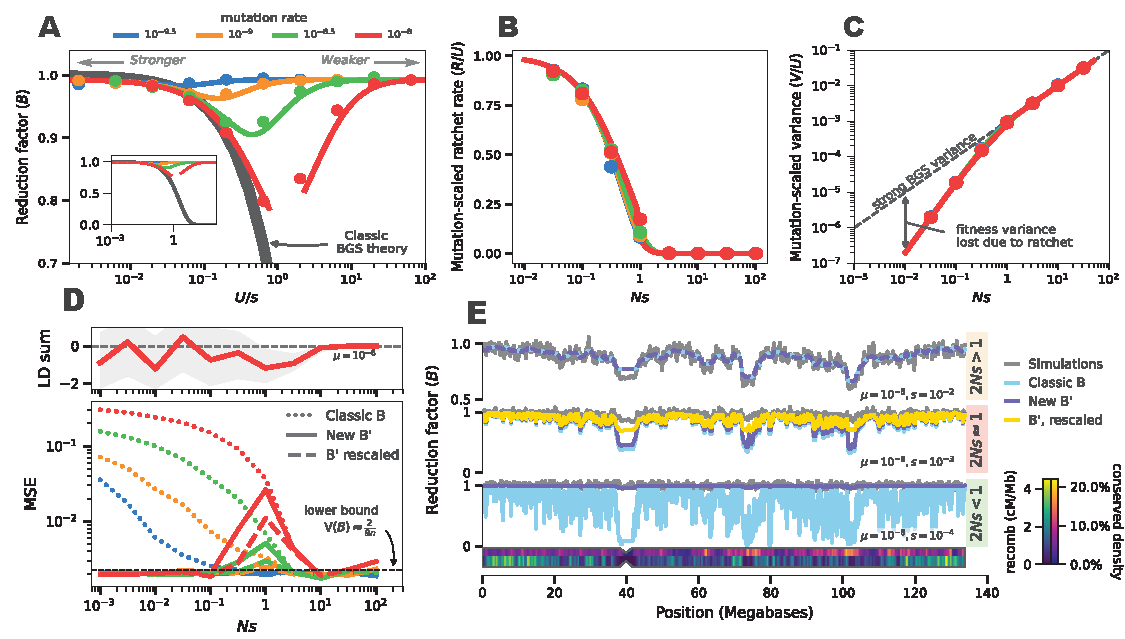
\includegraphics[width=\textwidth]{figures/figure_1.pdf} \caption{Theory
        compared to simulation results. (A) The predicted reduction factor
        under classic B theory (dark gray line) and the diploid SC16 model
        (colored lines corresponding to mutation rate) compared to average
        reduction across XXX simulation replicates (points). (B) The predicted
        ratchet rate under the SC16 model scaled by mutation rate (colored
        lines) compared to the ratchet estimated from simulation (points). When
        $2Ns>1$, the ratchet rate is near zero. (C) The genic variance from
        simulations (points) against the predicted variance under the SC16
        model (colored lines). As the ratchet begins to click, the genic
        variance is decreased from the level expected under strong BGS (dashed
        line). (D, bottom) The mean squared error (MSE) between
        whole-chromosome simulations and predicted classic B (dots), new B'
        (solid), and locally-rescaled B' (dashed) for different mutation rates
        (colors). The dashed horizontal line is the approximate theoretic
        minimum MSE. (D, top) The build up of negative linkage disequilibria
        around $2Ns=1$ in whole-chromosome simulations in bottom panel. (E) The
        average B map from 100 chromosome 10 simulation replicates (gray)
    against different predictions, for parameters that correspond to $2Ns < 1$,
$2Ns = 1$, and $2Ns > 1$. The chromosome shows the density of conserved sites
and recombination map used in simulations. }
  \label{fig:figure-1}
\end{figure}

Given that Santiago and Caballero's (\citeyear{Santiago2016-mu}) model is a
haploid-model for a single region under equilibrium negative selection, we
first sought to confirm it could accurately predict the reduction in realistic
forward-time simulations of diploid populations with recombination. Using SLiM
\parencite{Haller2019-vu,Haller2023-uk} we simulated a region of $10^5$
basepairs under varying levels of mutation and selection (see Methods
\ref{sec:methods-segsim}). We find a close correspondence between the observed
and predicted reductions in effective population size $B=\nicefrac{N_d}{N}$
over all selection and mutation parameters including weak selection (Figure
\ref{fig:figure-1}A), in contrast to classic BGS theory. Furthermore, to
investigate whether this accuracy was caused by the model correctly predicting
the equilibrium fitness variance and ratchet rate, we also measured these
throughout the simulation. Again, we find the diploid SC16 theory accurately
predicts both the ratchet rate (Figure 1\ref{fig:figure-1}B) and the genic
fitness variance (Figure 1\ref{fig:figure-1}C).

Moreover, these simulations provide intuition about the underlying negative
selection process. When mutations are strongly deleterious, there is no chance
they can fix, and the ratchet rate is zero (Figure \ref{fig:figure-1}B for $2Ns
> 1$). In this strong selection regime, the additive genic fitness variation
closely matches the theoretic deterministic equilibrium of $V_a = Us$ (dashed
gray line, Figure \ref{fig:figure-1}C) However, around $2N_e s \approx 1$, the
ratchet begins clicking as $p_F > 0$. When this occurs, each click of the
ratchet eliminates variation, and the equilibrium variation diverges from the
deterministic mutation-selection equilibrium (Figure \ref{fig:figure-1}C).

\subsection*{Chromosome-wide Simulations and Models of Negative Selection}

Given the accuracy of the SC16 model in predicting the reduction factor $B$ and
ratchet rate for a single segment under general mutation-selection processes,
we extended their model so that it could be applied to whole-genome data. Our
software method \texttt{bgspy} calculates the equilibrium additive genic
fitness variance ($V_a$) and ratchet rate ($R$) across grids of mutation rates
and selection coefficients for each pre-specified segment in the genome that
may be under negative selection (e.g. coding sequences or UTRs). Then, our
method computes a reduction map $B(x)$ for each position $x$ in the genome,
which is determined by the fitness variation at each segment and their spacing
along the user-supplied recombination map (see Methods XXX). To distinguish
between McVicker's B maps based on classic BGS theory, we call our reduction
map $B(x)$ a B' map.

To assess our predicted B' reduction maps, we simulated negative selection for
fixed mutation rates and selection coefficient on human chromosome 10 using
realistic recombination maps and conserved feature positions. Averaging over
$100$ replicates, we estimated the simulation expected reduction map and
compared this to the predicted B and B' maps for the same parameters. We find
that our B' maps and the classic BGS theory B maps closely match simulations
when selection is strong (top row of Figure \ref{fig:figure-1}E). This provides
the first realistic forward-time chromosome-scale simulation confirmation of
classic BGS theory. However, we find slight discrepancies in regions with low
recombination (Figure \ref{fig:figure-1}E). Second, we find our theory is
vastly more accurate than the classic B maps when selection is very weak ($2N_e
s \ll 1$; bottom row of Figure \ref{fig:figure-1}E), which is expected since
BGS theory does not work in this domain. Across all mutation and selection
parameters simulated, the relative error of the classic B maps is 14.6\%
whereas the relative error in the new B' maps is 5\%. Additionally, we find
that the mean squared error between simulations and B' maps is close to the
theoretic lower bound set by the coalescence variance \parencite[see Methods
XXX]{Tajima1983-gu}.

Nearly all of the error between the new B' maps and chromosome-wide simulations
occurs around the drift-barrier domain of $2Ns \approx 1$ (Figure
\ref{fig:figure-1}D). The higher error in this domain occurs across all
mutation rates. We hypothesized that the higher error in this domain may be
because when our method numerically solves Equations \eqref{eq:main_eqns} for
each segment, it does not consider the reduction experienced due to selection
at other linked segments. In particular, we use a fixed drift-effective
$N=1000$ corresponding to the number of diploids in the simulations rather than
$B(x) N$ at position $x$. To test this, we implemented a locally-rescaled
version of the B' maps, which numerically solves Equations \eqref{eq:main_eqns}
for each segment at position $x$ taking into account the reduction experienced
due to selection at other segments by setting $B'(x)N$ as the population size
(see Method XXX). We find the locally-rescaled B' maps reduce the relative
error from 5\% to 0.4\% and mean squared error (Figure \ref{fig:figure-1}D,
dashed colored lines), but does not entirely eliminate the error in the $2Ns
\approx 1$ domain.

Finally, we hypothesized that the remaining error is because of the build up of
negative linkage disequilibria between selected sites due to Hill--Robertson
interference \parencite{Hill1966-kd,McVean2000-bt,Comeron2007-wq}. To assess
this possibility, we calculated the sum of all linkage disequilibria in our
chromosome-wide simulations. We find negative linkage disequilibria build ups
around $2Ns \approx 1$ (Figure \ref{fig:figure-1}D, top row) and is stronger
when mutation rates are higher (Supplementary Figure XXX). As $Ns \to 0$, the
variance in LD inflates as expected \parencite{Ohta1969-ae,Hill1968-ue}.
Overall, the build up of negative LD is consistent our view that the
equilibrium fitness variance modeled by the SC16 theory is the additive
\emph{genic} fitness variance, which differs from the additive genetic variance
by the sum of linkage disequilibria between selected sites (i.e. $\delta_{LD} =
s^2 \sum_{i\ne j} D_{i,j}$ where $D_{i,j}$ is the LD between sites $i$ and
$j$). However, according to theory, the reductions in diversity should be
determined by levels of additive genetic fitness variance that include the
contribution of LD (Supplementary Materials Section XXX).

While we find evidence that local-recalling reduces error in the $2Ns \approx
1$ domain, we do not employ it in our genome-wide inference method for a few
reasons. First, the reduction map 

numerically solving the system of equations 

it currently cannot be used during when fitting
genome-wide models.

\subsection*{Application to Humans and Model Comparison}


Our method takes tracks of annotated features (an ``annotation model") that are
\emph{a priori} expected to have similar fitness effects, and estimates the
distribution of fitness effects for each feature type. We consider two classes
of annotation models: (1) CADD score models, which assign a rank-order
pathogenicity score to each basepair, and (2) and more interpretable gene
feature-based models that includes protein coding regions, intron and UTRs, and
PhastCons regions. We include PhastCons regions because there is abundant
evidence of highly-conserved non-coding regions in humans under negative
selection
\parencite{Meader2010-hm,Harmston2013-tt,Katzman2007-gq,Siepel2005-wh}, but
would not be included in gene-based annotation. Since our method fits a DFE for
each feature type, PhastCons regions that overlap other gene annotations (e.g.
coding sequences) must be assigned to either of the two feature types. Since
this can impact estimates, we fit both alternatives: a PhastCons Priority
model, where genic features that overlap PhastCons regions are classified as
PhastCons, and a Feature Priority model, where gene structure features take
priority and the PhastCons type catches all highly-conserved non-genic regions.
In total, we fit four annotation models (CADD 6\%, CADD 8\%, PhastCons
Priority, and Feature Priority) to high-coverage 1000 Genome data for three
populations: Yoruba (YRI), Han Chinese (CHB), and European (CEU) ancestries. We
assess and compare our models according to how well they predict patterns of
diversity on whole chromosomes left-out during the model fitting process. We
use the metric $R_\text{LOO}^2$, which is the proportion of the observed
variance in genomic diversity at the megabase scale predicted by our model. We
experimented with a few smaller spatial scales, but our results were consistent
with previous results suggesting the human linked selection signal fits best at
the megabase scale \parencite{Murphy2022-sj}.

\begin{figure}[htbp] \centering
    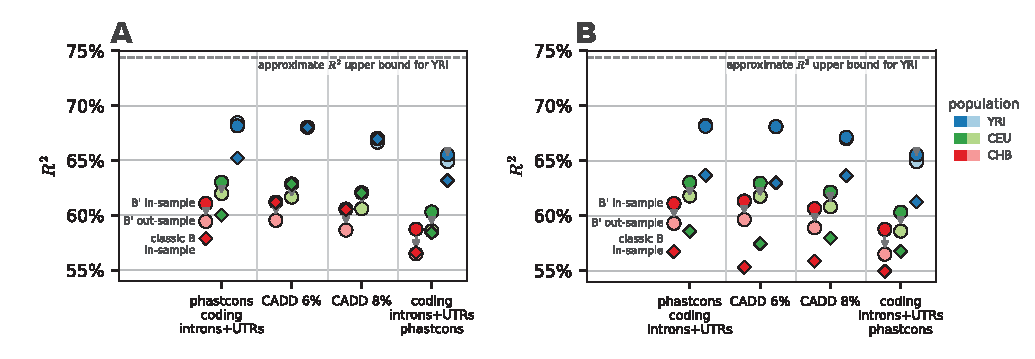
\includegraphics[width=\textwidth]{figures/figure_2.pdf} 
    \caption{The $R^2$ estimates for a sparse (A) and full (B) models, for all 
    populations (colors) fit at the megabase-scale. Round points are our B' 
    method and diamonds are the classic B. Lighter color round points are
    the out-sample $R_\text{LOO}^2$ estimates for our B' method, and arrows show the decline
    in goodness-of-fit due to in-sample overfitting (out-sample $R_\text{LOO}^2$ 
    were not calculated for classic B values due to computational costs). The 
    horizontal dashed lines are the $R_\text{drift}^2$ expected when the residual
    variance is given by the theoretic variance in coalescence times due to drift alone.}
  \label{fig:figure-2}
\end{figure}

Overall, we find the PhastCons Priority and CADD 6\% models fit about equally
as well (Figure \ref{fig:figure-2}A), explaining $R^2=68.45$\% and
$R^2=68.04$\% of the out-sample variance in Yoruba pairwise diversity at the
megabase-scale, respectively. In populations impacted by the out-of-Africa
bottleneck, the goodness-of-fit was lower across all models (e.g. 62.98\% and
59.98\% for CEU and CHB respectively in the PhastCons Priority model). The CADD
6\% model was previously found by \textcite{Murphy2022-sj} to be the
best-fitting model using classic BGS. Our PhastCons Priority model fits
marginally better than the CADD 6\% model consistently across all three
populations (Supplementary Table XXX). This is likely because the PhastCons
Priority model has more DFE parameters, and thus can fit finer-scale
differences in the DFE across its four feature types. By contrast, the CADD 6\%
track must fit patterns of diversity to conserved sites under a single DFE. The
CADD 8\% model fit slightly worse than the CADD 6\% across all populations, and
the Feature Priority model had the poorest-fit.

Since our method is built upon theory that fixes the weak selection problem of
classic BGS theory, it should in principle fit equally well when an annotation
model includes regions that are likely neutrally evolution. To test this, for
each annotation model (which are ``sparse") we fit a ``full" model that assigns
the remaining complement of the genome as a feature called ``other". This other
category is likely to predominantly neutrally evolving. Ideally, the
goodness-of-fit of model using our B' method should be invariant to whether an
annotation model is sparse or full. Indeed, we find this to be the case: both
in-sample $R^2$ and out-sample $R_\text{LOO}^2$ values are nearly identical
across full and sparse-track models (Figures \ref{fig:figure-2} A and B, round
points). 

By contrast, full annotation models fit poorly when using classic BGS theory
(Figure \ref{fig:figure-2}B, diamond-shaped points) and lead to unreasonable
parameter estimates (discussed below). Additionally, when sparse annotation
models contain genomic features that are likely under weak constraint (such as
introns and UTRs), models fit worse under classic BGS theory than our B' method
(Figure \ref{fig:figure-2}A). However, among the CADD annotation models, the
goodness-of-fit is nearly identical between B' and classic BGS methods. This
behavior is what we would expect given that the CADD annotation models contain
only the most pathogenic sites, which are \emph{a prior} very likely under the
strong selection domain under which B' and classic BGS theory agree.

Since our $R_\text{LOO}^2$ estimates suggest our models fit left-out
chromosomes well even though our method assumes constant demography and
homogeneous mutation rates along the genome, we wondered what $R^2$ we could
expect under a simple theoretic model where $\cov_i(B_i', \varepsilon_i) = 0$
and $\var_i(\varepsilon_i)$ was determined by the variance in neutral
coalescence times alone with an effective population size rescaled by $B_i'$.
We calculate this ``coalescence $R^2$" by calculating the theoretic coalescence
time variance in a megabase window with recombination and an effective
population size of $B_i' N_e$ where we use our best-fitting model's as a
plug-in estimator of $B_i'$. We note that this is a rough approximation, since
this calculation assumes constant demography and that the variance in
coalescence times under negative selection is likely lower than expected under
drift alone. 

Still, we find that our out-sample $R_\text{LOO}^2$ for Yoruba individuals
($R_\text{LOO}^2 \approx 68$\%) is close to the theoretic $R_\text{coal}^2
\approx 67$\%. For bottlenecked out-of-Africa populations, $R_\text{coal}^2
\approx 64$\% compared to the observed $R_\text{LOO}^2 \approx 62$\% for CEU
and $R_\text{LOO}^2 \approx 59$\% for CHB. We note that because bottlenecks
increase the variance in coalescence times beyond the level implied by the
effective population size, the disagreement between observed $R_\text{LOO}^2$
and the theoretic $R_\text{coal}^2$ is likely to shrink. Overall, this suggests
that negative selection models explain the vast majority coalescence time
variation at the megabase-scale that is capable of being explained (i.e. that
is not coalescence noise).

\subsection*{Estimates of Negative Selection Parameters in Humans}

\begin{figure}[htbp] \centering
    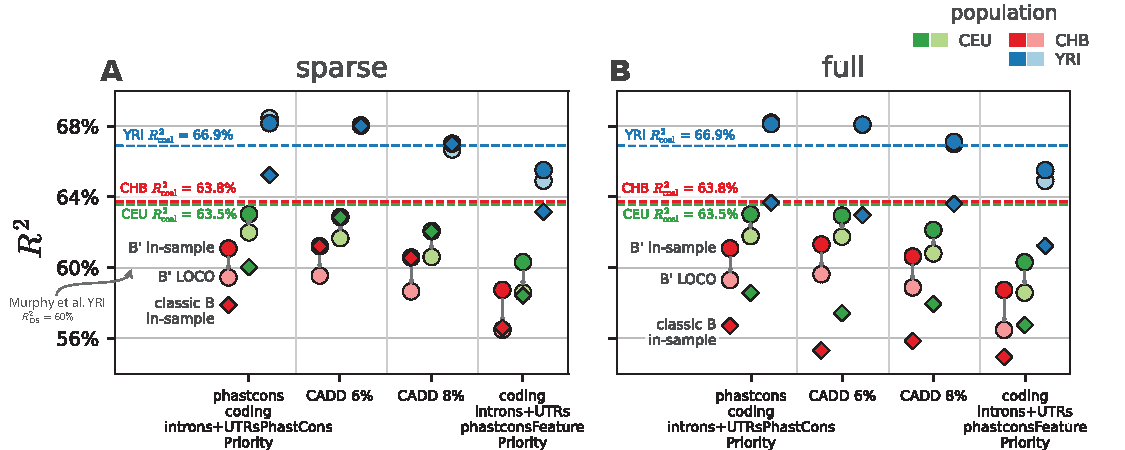
\includegraphics[width=\textwidth]{figures/figure_3.pdf} 
    \caption{The distribution of fitness effects of new mutations estimates for
        Yoruba individuals. (A) The DFEs using sparse (left column) and
        full-coverage (right column) tracks, across different annotation models
        (row). Color indicates the feature type. (B) The DFE of the
        full-coverage CDS-priority model comparing the estimates across
    populations.}
  \label{fig:figure-3}
\end{figure}



Next, we developed a composite-likelihood method to estimate pairwise diversity
in the absence of linked selection $\pi_0$, the deleterious mutation rate
($\mu_D$), and distribution of fitness effects ($\mathbf{W}$) under negative
selection. Because the focus of our work is to fix deficiencies in the classic
BGS model, our current implementation does not consider reductions in diversity
due to recurrent hitchhiking or other positive selection processes. Since
previous work has established that purifying selection is the dominant mode of
linked selection in humans and hitchhiking plays a limited role
\parencite{McVicker2009-ax,Murphy2022-sj}, humans are a suitable organism to
test our method. 

\begin{figure}[htbp] 
    \centering
    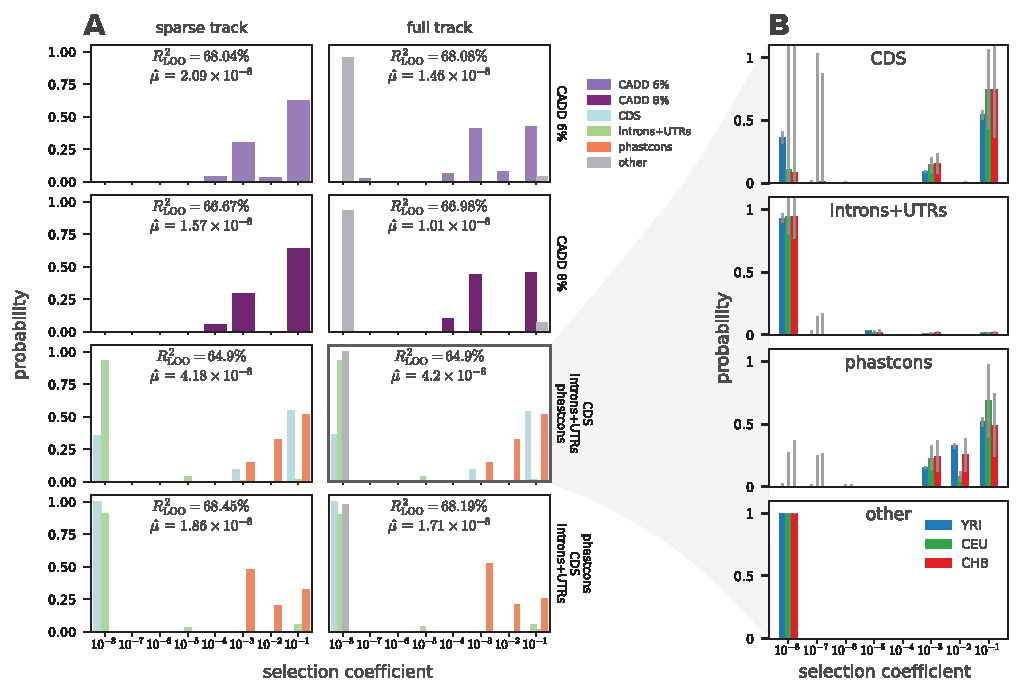
\includegraphics[width=\textwidth]{figures/figure_4.pdf} 
    \caption{}
  \label{fig:figure-4}
\end{figure}

Given that previous methods used classic BGS theory to fit genome-wide patterns
of human diversity, we were curious whether their qualitative findings would
change once weak selection was more accurately predicted. In particular, the
U-shaped relationship between $B'$ and the strength of selection suggests that
a given reduction factor could be explained by two different selection
coefficients.

\subsection*{Predicted Diversity Substitution Rates}

\begin{figure}[htbp] \centering
    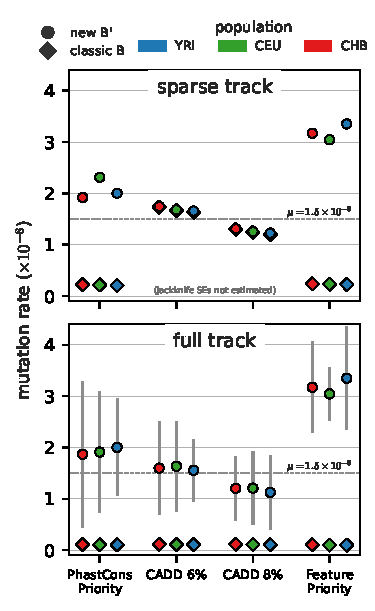
\includegraphics[width=\textwidth]{figures/figure_5.pdf} 
    \caption{}
  \label{fig:figure-4}
\end{figure}

When we fit our negative selection model to genome-wide patterns of diversity,
the parameter estimates generate three predicted quantities: (1) the $B(x)$
map, (2) the substitution rates per segment, and (3) the fitness variance per
segment. Here we focus on the predicted $B(x)$ map and implied levels of
diversity at the megabase scale. We discuss substitution rates and fitness
variance in the next section.

We also obtain a prediction $\widehat{B}_i$ for the reduction factor $B_i$ in
each window $i$, which can be multiplied by our estimate of $\widehat{\pi}_0$
to obtain a prediction of diversity $\widehat{\pi}_i = \widehat{\pi}_0
\widehat{B}_i$. 

\subsection*{Model Predictions and the Substitution Process}

Our method accommodates weak selection by modeling the fitness variance in each
segment under an equilibrium negative selection process. This fitness variance
is found by simultaneously solving for the per-generation substitution rate $R$
and the draft-effective population size $N_d$ for each segment. When our model
is fit to genome-wide diversity data, the parameter estimates imply predictions
of the deleterious substitution rate per basepair, per generation, for each
feature. Our method only considers within-species pairwise diversity, so these
predicted substitution rates constitute a test that our model is making
reasonable out-sample predictions of the substitution rates across features.

We focus specifically on the predictions from our feature-based annotation
models, since we can readily estimate human substitution distances for each
feature to compare to our predictions.

The estimated substitution distance should in theory equal the product of the
substitution rate per site, per year and the branch length in years.

When comparing our predicted mutation rates to observed substitution distances,
we must account for three major sources of uncertainty.

First, the split time between humans and chimpanzees is unknown, with estimates
ranging from 6Mya to 12Mya (XXX). Second, our predictions are in sites per
generation, and the appropriate human generation time is unknown. Third, the
appropriate mutation rate to use is debated, since there may have been a
mutational slow down on the human lineage (XXX), which could explain why
phylogenetic- and pedigree-based mutation rate estimates differ by roughly a
factor of two (XXX). Finally, we are only considering modeling the deleterious
substitution rate. In reality, some fraction of observed substitutions fixed
because they were beneficial. 





For a particular feature $f$, the estimated per-site substitution distance
$S_f$ along a branch (which accounts for back mutations) should correspond to
$S_f = T_g r_f$, where $T_g$ is the time in generations and $r_f$ is the
substitution rate per basepair, per generation of that feature. 

Each feature is
composed of basepairs with varying selection coefficients distributed according
to the feature-specific DFE vector $\mathbf{w}_f$ and corresponding vector of
substitution rates per selection coefficient, $\mathbf{r}_f$.

Our estimate of a feature's DFE
is $\widehat{\mathbf{w}}_f$.

We calculate the 


\begin{align}
    \label{eq:sub}
    r_f = \mu \int_0^1 p_F(s) ds
\end{align}

Solving the XXX equations, we end up with predictions $\widehat{r}_f$ for the
per-basepair, per-generation substitution rate for each feature. These are
calibrated to the MLE mutation rate estimate $\widehat{\mu}_\text{del}$, which
as mentioned, excludes the contribution of lethal mutations which act purely to
reduce $N_e$ and thus only impact $\pi_0$. Using Equation \eqref{eq:sub} we can
re-calibrate these estimates against other mutation rates. 

Because of it's greater interpretabilty, we initially focus on the substitution
rate estimates from the Feature Priority model even though it had a poorer-fit
and high mutation rate estimate. 

We can also re-calibrate this model to an alternate mutation rate.

% - Table s5 https://oup.silverchair-cdn.com/oup/backfile/Content_public/Journal/genetics/206/1/10.1534_genetics.116.197145/8/files1.pdf?Expires=1686357613&Signature=cp9qoI2ChCb6GFZ74HI4eWcA~MQ4sHlWyeI3Zp49-5xEORzMfYlSRxzVvZlo8ZoGWDi0G3PnL00ZplM-~or4YIVm2uhkmqjf61AmC7RdZ1QTak4j0kFMQ0wAbM9pusiV3gIepTQHq2HKRKwgS~ypmv~0oqO5dDxaq9nhOWIBBmLAA49oHWuxUtnRe3sEYATwCwjIFEomhgJpg7vKGCF~87GdCV4JETW4PN2VvD4hsu2AVRd8yA~vUJvsXfhWwcElDeY4fsgpprl1lC3XGjJCnqdwbzRGPV5LNx5XEKLptcZtLeLcOmFJCvmVLe0bewJ7Vta0TSQM7T9AuklompjPPw__&Key-Pair-Id=APKAIE5G5CRDK6RD3PGA

Like other methods, our method divides the putatively conserved basepairs up

Generally, when the putatively conserved region is larger, there is a tradeoff
in two dimensions. First, more bases are conserved according to the same DFE,
so the total mutational load increases. This causes the tradeoff between
mutation rate estimate and CADD fraction we observe across both our B' model
and the classic B when using sparse tracks (Figure 2XXX). 


We find that mutation rate estimates are fairly sensitive to model choice
(Figure 2XXX). 

Since B' has a U-shaped relationship with the selection coefficient, we
hypothesized that our model may reveal true identifiability issues in
estimating the DFE that do not occur under the classic B model. We find that
this is not the case for our models fit at the megabase-scale. The DFE
estimates for our CADD6 and CADD8 models are consistent (Figure XXX), and both
produce similar mutation rates.

While we do not comprehensively fit all of our model to other spatial scales,
we 

However, while a given reduction level may be explained by either a weak or
strong selection coefficient, the spatial extent of these reductions caused by
weak selection is much narrower than under strong selection. 

We see evidence this is the case in several of our models, where
genome-wide diversity fits equally well between models with mutation rates 

Indeed, we see this by comparing parameter estimates of the CADD6
sparse-track model using classic BGS B and our B' method. 


(which mimics the best-fitting model of
\cite{Murphy2022-sj}) 

(see also
Appendix 1, Figure 26A of \cite{Murphy2022-sj})

correlation between s and feature

Overall, we find evidence that negative selection models are very sensitive to
the input track. Because inference based on our B' method accommodates weaker
selection, the primary models we fit here more robust to misspecification of
the regions

\subsection*{Evolutionary Models}

We model the diversity at punitively neutral sites. These are sites in regions
we have \emph{a prior} reason to believe have a DFE nearly entirely
concentrated in the neutral range. While this may not be the case in reality,
it is necessary given the computational demands of modeling whole-genome
selection. 

CDS+phastcons+UTR model

 - UTR as neutral control

 - CDS takes priority over phastcons, phastcons is fallback. Otherwise, the
   effect of CDS would be biased by the fraction removed and classified as
   phastcons. This is the right comparison for the substitution model.

\subsection*{Predicted Substitution Rates}

- mention neg. auto correlation?

- Gene level analysis

To evaluate the predicted substitution rate of our CDS+phastcons+UTR model, 


Additionally, our GBGS model makes predictions about the rate of substitutions
in different segments under purifying selection. There are two stages of the
prediction process. First, when the initial B' maps are calculated, the
predicted substitution rate is calculated as a byproduct of 

\section*{Discussion}

It is worth considering why this model performs well for models of negative
selection. The fitness variance equation, $V(x) = (U-2R)s$ tells us that under
models, the long-run variance is set by the balance of mutation and fixation.
Whether a particular basepair's behavior follows this equation depends upon
whether the long-run average is close to ``typical" for that basepair at a
given time. Good things fix so quickly, that we're left with a constant
churning of new variation

- need for coalescent simulations with reduced $N_e$ along the genome.

- we need to talk about Fisher's Fundamental Theorem and how this model
connects fitness variation to absolute changes in fitness.

Measuring selection in the Genome Versus Finding Selection in the Genome


\section*{Methods}
% (the method would support a new
% ``interaction" type, but this greatly increases the number of parameters).

\subsection*{Solving the B' Equations for each Segment}
\label{sec:methods-bprime-eqns}

Our software \texttt{bgspy} first calculates the equilibrium additive genic
fitness variation $\widetilde{V}_a$ and ratchet rate $\widetilde{R}$ for each
user-specified segments in the genome. These equilibria are calculated across
grids of mutation rate weighted by the DFE $m_i$ and selection coefficient
$s_j$, by numerically solving the following system of equations,

\begin{align}
  \label{eq:}
  {N}_{d} &= N \exp \left( -V_a \frac{Q^2(m_i, s_j)}{2} \right) & \text{\emph{effective population equation}} \\
  R &= \frac{4N_dU s_j}{\exp(4 N_d s_j)-1}  & \text{\emph{substitution equation}} 
\end{align}

where,

\begin{align}
  %V(x) &= U s - 2 {R}(x) s & \text{\emph{fitness variance equation}} \\
  V_a &= (U - 2 R) s_j & \text{\emph{fitness variance equation}} \\
  Q^2(m_i, s_j) &= \frac{2}{(1-Z)(2-(2-M)Z)} & \text{\emph{linkage inflation factor}} \\
  Z &= 1 - \frac{Us_j}{U-{M}} & \text{\emph{variance decay rate}}
\end{align}
%
and $U = m_i L$ and $M = r_\text{BP} L$ are the total mutation and
recombination rates in the segment. A detailed derivation of these equations
can be found in Supplementary Section \ref{suppsec:theory}. The recombination
rate in a segment is determined by a user-supplied recombination map.

\subsection*{Calculating the Reduction Maps}
\label{sec:methods-maps}

Our method uses the pre-computed equilibria $\widetilde{V}_{a,g}$ for each
segment $g$ to calculate the reduction map $B(x; m_i, s_j)$ at positions $x$
across the parameter grids described above. Since we assume multiplicative
fitness, the reduction is the product of each segment's contribution accounting
for the recombination is,

\begin{align}
    B(x; m_i, s_j) = \exp\left(- \frac{1}{2}\sum_{g \in G} \sum_{i=1}^{n_s} \widetilde{V}_{a,g}(m_i, s_j) Q_g^2(m_i, s_j, r_{x, g})\right)
\end{align}
%
where $r_{x, g}$ is the recombination fraction between the focal site and
segment $g$. Here, $Q^2(m_i, s_j, r_{x,g})$ is given by Equation \eqref{eq:Q}
squared. A separate reduction map is calculated for all features $G$ within a
specific feature type. We calculate B' calculate for $\log_{10}$-spaced grids
over $10^{-1} \le s \le 10^{-8}$ and $10^{-11} \le m \le 10^{-7}$, in 10kb
increments across the genome.

\subsection*{Composite Likelihood and Optimization}
\label{sec:methods-likelihood}

Following previous approaches
\parencite{McVicker2009-ax,Elyashiv2016-vt,Murphy2022-sj}, we use a composite
likelihood approach to fit our negative selection model. Per-basepair allele
count data (described below) is summarized into the number of same and
different pairwise differences per window. All of our primary models were fit
with megabase windows, since previous work has found the strongest selection
signal at this scale (we confirm this with one XXX fit at the $10^5$bp scale).

We use a binomial likelihood with probability $\bar{\pi}(b; \Psi) = \pi_0
\bar{B}(b; \mu, \mathbf{W})$, where bars indicate averages over some bin width.
With multiple features classes and a map $k(g)$ between a segment $g$ to its
class, the reduction map is,

\begin{align}
    \log\left(B(x; W, s_j) \right) = - \frac{1}{2} \sum_{g \in G} \sum_{i=1}^{n_s} V_g(\mu W_{j, k(g)}, s_j) Q_g^2(m_i, s_j, r_{x, g}).
\end{align}

Here, $\mu$ is the mutation rate and $\mathbf{W}$ is the $n_s \times K$ DFE
matrix over the selection grid and features. Since each column of the DFE
$\mathbf{W}$ must sum to one, numeric optimization was done in unconstrained
$n_s-1$ dimensional softmax space. Our binomial likelihood modeled the number
of different pairwise comparisons observed per window given the predicted
pairwise diversity and total number of comparisons implied per window (see
Supplementary Materials Section \ref{supp:data-summary}).

We tested multiple different optimization routines, finding that BOBYQA
outperformed alternatives \parencite{Powell_undated-ec}. We inspected and
confirmed convergence with diagnostic plots finding stable optima across 10,000
random starts (see Supplementary Materials Section XXX).

\subsection*{Segment Simulations}
\label{sec:methods-segsim}

To assess the accuracy of the SC16 theory, we conducted forward simulations
across grids of mutation rates ($\log_{10}(\mu) = \{10^{-9.5}, 10^{-9}, \ldots,
10^{-8}\}$) and selection coefficients ($\log_{10}(\mu) = \{-1, 1.5, 2, \ldots,
4.5\}$) using SLiM \parencite{Haller2023-uk,Haller2019-vu}. Each simulation
evolved a 100kb region with deleterious mutations entering at rate $\mu$
per-basepair, per generation, each with an additive selection coefficient of
$-s$. Total fitness was multiplicative across sites. Each simulation recorded
the number of fixations and the fitness variance per generation. After $10N$
generations, the ARG of the tree was recorded and downstream Python scripts
calculated diversity in the center of the region. We averaged the results of
$10,000$ replicate simulations to compare against theory.

\subsection*{Chromosome-wide Simulations}



, using the HapMap recombination map (XXX) and in coding regions, PhastCons
regions, and UTRs as an approximate set of putatively conserved segments

We calculate the mean squared error (MSE) and relative error between
whole-chromosome simulations and the predicted B and B' maps by averaging
branch diversity in 10 kilobase windows (tskit, XXX) and dividing by the
neutral expectation of $4N$. The theoretic lower bound of the MSE is due the
noise in estimating the expected reduction map from simulations. For $n=100$
replicates, the sampling noise is minimal relative to the evolutionary noise in
the coalescence process \parencite{Tajima1983-gu}. We use this as the theoretic
lower bound assuming the maximum coalescence noise at $B=1$, $\var(\bar{B})
\approx \nicefrac{2}{9n}$.

\subsection*{Human Population Genomic Diversity Estimates}

We estimate pairwise diversity for Yoruba (YRI), European (CEU), and Han
Chinese (CHB) ancestry individuals in the high-coverage 1000 Human Genomes
dataset (XXX). We 

\subsection*{Local-rescaled }
We note that it is computationally intractable to solve this equation excluding
the contribution of the focal segment 

\subsection*{Assessing the B' Maps}

We first assessed the B' maps against the observed average reduction across
$XXX$ forward-simulations, $\bar{B}_\text{sim}(x)$. The mean-squared error has
two sources, (1) bias from a breakdown in our theory $B(x)$ for the average
reduction, and (2) variance from the simulations. We show that for most of the
parameter space, the measured mean-squared error between simulation averages
and our B' maps is at the theoretic minimum. This minimum variance is entirely
from the coalescent noise when estimating $\bar{B}\text{sim}(x)$, which 

\subsection*{Maximum Likelihood Estimation}

\subsection*{Local Rescaling and Substitution Rate Prediction}


\subsection*{Substitution Rate Predictions}

Our MLE fit $\hat{\Phi}$ also implies a set of corresponding substitution rate
predictions for each segment under mutation-selection-draft process. There are
two sources of variation in these predictions in this model. First, there is
the variation across the pre-specified functional categories, e.g. CDS, UTRs,
and PhastCons. Second, there is region-specific variation 









% As genomes are transmitted through the generations, lifetime events selectively
% alter what is passed to the next generation. While selection directly acts on
% the genetic variants that cause heritable fitness differences among
% individuals, neighboring regions experience an indirect contraction in genetic
% variability. This byproduct is known as \emph{linked selection}, and it occurs
% when selection changes a site's frequency on timescale faster than
% recombination can decouple that site from its genetic background. Because
% linked selection modifies the genetic variability in a regionally-correlated
% way, it creates observable patterns in genomic data that are used to understand
% the type of selection processes acting on genomes and estimate key evolutionary
% quantities. 

% , with characteristic length
% $\nicefrac{s}{r}$ basepairs, where $s$ is the heterozygous selection
% coefficient and $r$ is the per-basepair recombination rate. Sweeps were found
% in humans, \emph{Drosophila}, and other species (XXX), though it was unclear
% whether hitchhiking alone could explain the observed genome-wide correlation
% between recombination rate and genetic diversity in some species (XXX). 

% Much work has been done on developing mathematical theory for two linked
% selection processes: hitchhiking and background selection. These are
% distinguished by the evolutionary processes that generate fitness variation and
% the resulting selection dynamics. Under the classic hitchhiking model, a new
% beneficial mutation sweeps fixation, leading to a dip in genetic diversity on a
% small spatial scale. Since the sweeps leave relatively narrow footprint, they
% influence genome-wide diversity only when beneficial mutations are recurring
% and recombination is relatively limited, as in \emph{Drosophila}. These models
% assume sweeps are sufficiently rare as to not occur simultaneously, which is
% consistent with the slow estimated rate of strongly beneficial mutations (XXX).
% Overall, the classic hitchhiking model is simple because the underlying
% selection process does not generate polygenic fitness variation, even though
% this is type of variation plays a dominant role in adaptation (XXX).

% By contrast, background selection is a consequence of the fitness variation
% created by a steady influx of new deleterious mutations. The classic background
% selection model (XXX) considers how the balance between mutation introducing
% deleterious variants into the population and selection removing them, reduces
% nearby genetic variability. A critical assumption of this model is that such an
% equilibrium between mutation and selection exists, which is the case only when
% these mutations have a large enough fitness cost to ensure that they cannot fix
% in the population. Under this process, the number of deleterious mutations per
% gamete reaches a Poisson stationary distribution with rate $\nicefrac{U}{s}$,
% where $U = \mu_D L$ is the deleterious mutation rate ($\mu_D$ per basepair per
% generation) in a region of $L$ basepairs for mutations with a heterozygous
% selection coefficient of $s$ (XXX). The fraction of gametes without any
% mutations is then $f_0 = \exp(-\nicefrac{\mu_D}{s})$. Without recombination,
% any gamete with deleterious mutations is destined to bring its linked neutral
% variation with it to extinction, effectively reducing diversity levels to those
% expected in a neutrally-evolving population of size $f_0 N$. 

% Remarkably, predictions from simple background selection models with
% recombination closely match large-scale patterns of human diversity and
% divergence (XXX). Since background approximately rescales a neutral coalescent
% process by $f_0$, the predicted diversity is reduced from neutral levels by a
% factor $B = \nicefrac{N_e}{N}$, which is the ratio of effective population size
% under background selection to the population size. In background selection
% models with recombination, $B$ is determined by the number of conserved
% basepairs and recombination in a region. Consequently the predicted reduction
% along the genome (known as $B$ maps) mirror the regional density of conserved
% elements under purifying selection and recombination rates. These $B$ maps have
% been used in studies of XXX, are inputs into machine learning models that
% predict functional constraint, and XXX. Furthermore, since new deleterious
% mutations are perpetually flowing into populations $B$ maps may provide a
% better null model for evolution than the standard neutral model.

% While background selection models do predict diversity levels  XXX

% % outline?
% - Disentangling evolutionary processes from the patterns of genetic variation
% across the genome. The structure of what can be under selection shapes these
% patterns when selection acts; when drift acts, these patterns should not exist.

% - For species with small effective population sizes (and perhaps large map
% lengths), BGS seems to be a dominant selective force in shaping patterns of
% diversity (e.g. at the megabase scale in humans).

% - However, current approaches to fitting BGS models fail under the weak
% selection domain. This weak selection domain is important (discuss
% HRI/ratchet/etc). Importantly, the characteristic scale of the impact of linked
% selection is $\nicefrac{s}{r}$, meaning weak selection acts on smaller scales
% than strong selection. Our ability to see selection at small scales may be
% inhibited by the fact that our current BGS theory only works for strong
% selection.

% - We need to say briefly that we're using BGS to mean linked selection due to
% purifying selection, and thus the strong and weak regimes (classically it has
% just meant the strong regime).

% \section*{Conclusion}

% - care should be taken applying these methods to \emph{Drosophila}, since the
% $\delta_{LD}$ term could be much larger.

% \section*{Results}

% \subsection*{Theory}

% - overview of why BGS models fail?


% From an evolutionary perspective, linked selection is important because by
% modifying neighboring levels of genetic diversity, it is also directly altering
% the selection dynamics at these neighboring sites. 


% The other use of these models is to understand how linked selection processes
% differentially alter the genetic variability, or equivalently, the genealogical
% trees, along the genome. 

% XXX how many sites are under selection at any moment? What's fitness variation?



% Early on, some pointed out that evidence of strong selective sweeps in the
% human genome was not the full story 

% Generally, in organisms with large amounts of recombination, linked selection
% has 


% Weak selection processes 

% distorts
% genome-wide 

% diversity.

% The linked selection literature has primarily focused on developing theory for,
% and quantifying the effects of two linked selection processes: hitchhiking and
% background selection. Genome-wide models of the hitchhiking process consider
% how beneficial mutations that sporadically enter the population 

% - QGLS polygenic linked selection

% - H and W

% - inflation factor

% \subsection*{Statistical Methods}


TODO we need to make appoint about how Ben G's paper found the V(n)->VA connectoin -- this is their patching model

TODO we need to give some intuition for what Vm and V are in humans, e.g. back of envelope type stuff

% The $N_{e,t}$ terms are analogous to an instantaneous coalesce rate at
% generation $t$, which can be expressed in terms of the variance in allele
% frequency change by noting that in an ideal Wright--Fisher population,

% \begin{align}
%   \V(x_t) &= p_0(1-p_0) \left[1 - \left(1 - \frac{1}{2N}\right)^t \right]
% \end{align}




% This is an asymptotic $N_e$, but this does not accurately describe the levels
% of diversity (\cite{Santiago1998-bs} equation 16, \cite{Santiago2016-mu}
% equation 4).

% \begin{align}
%   \V(x_t) &= \V(x_1) \left(1 + \sum_{i=1}^t \left(1 - \frac{1}{2N}\right)^{i} \right) + \sum_{i \ne j} C_{i,j}
% \end{align}




% In general, the variance in allele frequency after $t$ generations
% of neutral evolution is,

%\begin{align}
%  \label{eq:var_freq}
%  %\V(x_t) &= \frac{x_0(1-x_0)}{2N}\left(\sum_{i=1}^t \left(1 - \frac{1}{2N}\right)^{i-1} \right)
%  \V(x_t) &= \V(x_1) \left(1 + \sum_{i=1}^t \left(1 - \frac{1}{2N}\right)^{i} \right)
%\end{align}






% Each term is time-indexed because it is conditioned on the starting neutral
% frequency in each individual, $x_{0,1}$. This equation is very general, and
% allows for any reproduction model with finite offspring variance and can
% account for the impact of linked selection under a variety of selection
% processes. 



% Next, we can partition the gamete number into heritable ($f_i$) and
% non-heritable ($\varepsilon_i$) fitness components of each individual $i$, $k_i
% = f_i + \varepsilon_i$. We define $f_i$ such that $\nicefrac{1}{N} \sum_i f_i =
% 2$ in a constant population, and $\varepsilon_i$ is noise term centered around
% zero. Then, the neutral allele frequency change is can be written as the sum of
% three independent stochastic terms,

% \begin{align}
%   \Delta p_1 &= \frac{1}{2N} \sum_{i=1}^N x_{0,i} (f_i - 1) +
%                \frac{1}{2N} \sum_{i=1}^N x_{0,i} \varepsilon_i
%   + \frac{1}{N} \sum_{i=1}^N \sum_{j=1}^{k_i} \delta_{0,i,j} \\
%   % \Delta p_1 &= \frac{1}{2N} \sum_{i=1}^N x_{0,i} (f_i - 1) +
%                % \frac{1}{2N} \sum_{i=1}^N x_{0,i} \varepsilon_i
%   % + \frac{1}{N} \sum_{i=1}^N \sum_{j=1}^{k_i} \delta_{0,i,j} \\
%   \Delta p_1 &= S_1 + D_1 + H_1
% \end{align}


% (c.f. \cite{Santiago1995-hx} equation 2 and \cite{Buffalo2019-qs} equation 30).

% Each term is time-indexed because it is conditioned on the starting neutral
% frequency in each individual, $x_{0,1}$. This equation is very general, and
% allows for any reproduction model with finite offspring variance and can
% account for the impact of linked selection under a variety of selection
% processes. 

% Now, let us look the variance of $\var(\Delta p_1)$ over evolutionary
% replicates.

% \begin{align}
%   \var(\Delta p_1) &= \var(S_1) + \var(D_1) + \var(H_1)
% \end{align}

% To introduce how this equation can be used to quantify the variance in allele
% frequency change through time, $\var(p_t - p_0$ for $t > 0$, we first look at
% evolution in a neutral Wright--Fisher model. Neutrality ensures that $S_t = 0$
% for all $t$.





%%% OLD

%There has been considerable past work to find both the rate of the ratchet
%(XXX), and summaries of the genealogies created under weak purifying selection
%(XXX). Our approximation combines a few theoretic avenues from past work. Our
%primary goal is to find a theoretic scaling function $B$ that rescales the neutral
%pairwise coalescent times the appropriate amount to 

%Strictly speaking, there is no way to rescale the coalescent under general
%background selection process, as genealogies deviate from the Kingman
%coalescent slightly under strong selection
%\parencite{Walczak2012-fi,Cvijovic2018-vd} and greatly under weak selection
%\parencite{OFallon2010-my}

%First, we approximate the coalescent effective population size, which
%determines expected pairwise diversity, from the variance effective population
%size. Then, we use a general quantitative genetic model of linked selection to
%find the variance effective population size under background selection. Since
%the impact of selection under this model is parameterized by the additive
%genetic fitness variance, we use an approximation for this based on the
%additive \emph{genic} variance, which depends on the rate of the ratchet.
%Previous work has been unable to find a simple closed-form solution to the rate
%of the ratchet because it depends on moments of the fitness distribution (e.g.
%fitness variation), which in turn depend on even higher-moments of the fitness
%distribution (e.g. the skew of the fitness distribution). While the ratchet
%should scale with the probability of fixation, the probability of fixation
%(Kimura, Malecot, XXX) is not accurate when multiple deleterious mutations are
%segregating simultaneously and in close linkage with one another. A key insight
%of \textcite{Santiago2016-mu} was that the classic equation for the probability
%of fixation is fairly robust as long as the correct effective population size
%is used. Their approach is to solve a system of two non-linear equations: one
%for the variance effective population size (which depends on the rate of the
%ratchet), and another for the time to fixation (which depends on the effective
%population size).

%Below, we step through the theory we use in our statistical methods. We
%re-derive central parts to illustrate where approximations have been made,
%which allows us to understand how these approximations may impact our
%statistical methods and inspect model fit in regions where these approximations
%are less likely to hold.

%\subsection*{Pairwise Diversity under Background Selection}

%The central quantity of interest for our statistical inference methods is
%average pairwise diversity along the chromosome. While other summaries of the
%data, such as the allele frequency spectrum, may be more informative about the
%evolutionary processes acting in a region, we lack population genetic theory
%for these quantities under most selective regimes and they require more degrees
%of freedom to characterize. By contrast, neutral diversity under an
%infinite-sites model is determined only by the per-basepair mutation rate $\mu$
%and the expected pairwise coalescent time $\E[T_2]$,

%\begin{align}
%  \E(\pi) = 2 \mu \E(T_2)
%\end{align}

%Let us assume that there is a constant \emph{drift-effective} population size
%$N_d$ which determines the rate of coalescence due only to neutral demographic
%processes. Additionally, we assume some background selection process that in
%expectation scales the effective population size by $b(t)$ at time $t$ (though
%this could in theory be due to any process). Then, the expected pairwise
%coalescent time is

%\begin{align}
%  \label{eq:T_2}
%  \E(T_2) = \sum_{i=1}^\infty \frac{i}{2 b(i) N_d}\prod_{t=1}^{i-1} \left(1-\frac{1}{2 b(t) N_d}\right).
%\end{align}

%The time-dependency of $b(t)$ is required because the background selection
%process will usually alter the rate of coalesce through time. For example,
%under weak and intermediate selection, coalesce rates speed up as lineages move
%in the past under intermediate to weak selection, similar to population growth
%\parencite{Walczak2012-fi,Seger2010-rs,Good2014-yz}. 

%% Intuitively, this is
%% because lineages are unlikely to coalesce with numerous less fit lineages they
%% encounter as they go back in time, until ultimately coalescing in one of the
%% least-loaded fitness classes. 

%This formulation is general and classic background selection theory (in the
%no-ratchet domain) is a special case of it. Under classic BGS and load theory,
%two randomly sampled lineages will each carry a number of deleterious mutations
%sampled from a Poisson stationary distribution. Because any lineage carrying $j
%> 0$ strongly deleterious mutations is destined to extinction, these lineages
%can only coalesce in a common ancestor in the least-loaded class with zero
%deleterious mutations. Under the Poisson stationary distribution, the size of
%this class is $f_0 N$, where $f_0 = e^{-\nicefrac{U}{s}}$, so the coalescent
%rate is scaled by $\nicefrac{1}{f_0}$. Once the lineages reach this fitness
%class, there are no fitness differences among individuals, so they coalesce
%following the Kingman process. A lineage moves backwards in time $t_d$
%generations through the ``delay phase" to the least-loaded class. Classic BGS
%theory ignores this delay phase, since $t_d \sim \log(j+1)/s << f_0 N$
%(Durrett, p. 213). 

%%Here, we model the background selection process forward in time. We approximate
%%the expected pairwise diversity with the probability of heterozygosity,
%%$\E(\pi) \approx \mathcal{H}$, which holds under weak mutation and random
%%mating, such that

%%\begin{align}
%%  %\mathcal{H} =  2 \mu \sum_{i=1}^\infty \prod_{t=1}^i \left(1-\frac{1}{2 b(t) N_d} \right)
%%  \mathcal{H} &= 1 - \sum_{i=1}^\infty (1-\mu)^{2i} \prod_{t=1}^i \left(1-\frac{1}{2 b(t) N_d} \right) \\
%%              &\approx 2 \mu \sum_{i=1}^\infty \prod_{t=1}^i \left(1-\frac{1}{2 b(t) N_d} \right)
%%\end{align}

%%in the limit where $\mu \to 0$. This is equation 4 of
%%\textcite{Santiago2016-mu}; they define the sum as the heterozygosity effective
%%population size.

%\subsection*{Forward in Time Models of Linked Selection}

%Next, show how quantitative genetic models of linked selection
%\parencite{Robertson1961-ho,Santiago1995-hx,Santiago1998-bs,Santiago2016-mu}
%find expressions for $b(t)$ with by modeling the selective process forward in
%time. Their approach is to consider how the variance in neutral allele
%frequency change is impacted by a linked selection process. 

%\subsubsection*{Variance in Neutral Allele Frequency in a Neutral System}

%For comparison, we start with the recursion for the variance in allele
%frequency change in a neutral Wright--Fisher model. Under binomial sampling of
%alleles, the random frequency $x_t$ is $2N x_t \sim \mathrm{Binom}(x_{t-1},
%2N)$. If we look forward in time on generation and treat $x_0$ as fixed,

%\begin{align}
%  \V(x_1) = \E_1\left[(x_1 - x_0)^2\right]= \frac{x_0(1-x_0)}{2N},
%\end{align}

%and

%\begin{align}
%  \V(x_2) &= \E\left[(x_2 - x_0)^2\right] \\
%          &= \E_1\left[\E_2\left[((x_2-x_1) + (x_1 - x_0))^2 | x_1\right]\right] \\
%          &= \E_1\left[\E_2\left[(\Delta x_2 + \Delta x_1)^2 | x_1\right]\right] \\
%          &= \E_1\left[\E_2\left[{\Delta x_2}^2|x_1\right]\right] + 2\E_1\left[\E_2[\Delta x_2 \Delta x_1 | x_1]\right] + \E_1\left[ {\Delta x_1}^2\right] \\
%          &= \E_1\left[\E_2\left[{\Delta x_2}^2|x_1\right]\right] + \E_1\left[ {\Delta x_1}^2\right] \\
%          &= \frac{x_0(1-x_0)}{2N}\left(1 - \frac{1}{2N}\right) + \frac{x_0(1-x_0)}{2N}
%\end{align}

%Note that the cross-moment $\E_1\left[\E_2[\Delta x_2 \Delta x_1 | x_1]\right]
%= 0$ under neutral evolution. In general, the variance in allele frequency
%after $t$ generations of neutral evolution is,

%\begin{align}
%  \label{eq:var_freq}
%  %\V(x_t) &= \frac{x_0(1-x_0)}{2N}\left(\sum_{i=1}^t \left(1 - \frac{1}{2N}\right)^{i-1} \right)
%  \V(x_t) &= \V(x_1) \left(1 + \sum_{i=1}^t \left(1 - \frac{1}{2N}\right)^{i} \right)
%\end{align}

%This geometric series converges to the familiar expression,

%\begin{align}
%  \V(x_t) &= x_0(1-x_0)\left(1 - \left(1 - \frac{1}{2N}\right)^t \right).
%\end{align}

%which in the limit $t \to \infty$, converges to the Bernoulli variance
%$x_0(1-x_0)$ as the frequency either goes to 1 with probability $x_0$ or 0 with
%probability $1-x_0$.

%% Now, if the effective population size were to change each generation, equation
%% \eqref{eq:var_freq} would be,

%% \begin{align}
%%   \V(x_t) &= \V(x_0) \left(1 + \sum_{i=1}^t \prod_{j=1}^{i} \left(1 - \frac{1}{2N(j)}\right) \right)
%% \end{align}

%% Note that this too converges to $x_0(1-x_0)$ as $t \to \infty$.

%\subsubsection*{Variance in Neutral Allele Frequency with Linked Selection}

%Note that equation XXX is a special case, when the evolutionary process has
%independent allele frequency changes through the generations and thus the
%cross-moment is zero. Selection generates correlations between allele frequency
%changes at nearby neutral sites. These correlations created by linked selection
%inflate the variance in neutral allele frequency $\V(x_t)$ beyond what it would
%be in a system without linked selection operating. The magnitude of this
%inflation term is set by the selection process and its dynamics, linkage
%disequilibrium, and the recombination rate. Even k




%The theory of this began with \textcite{Robertson1961-ho},
%and was thoroughly worked out by Santiago and Caballero
%(\citeyear{Santiago1995-hx}, \citeyear{Santiago1998-bs}; see also
%\cite{Barton2000-zg} and \cite{Buffalo2019-qs}). Our BGS statistical methods
%employ the extension of this model for weak BGS \parencite{Santiago2016-mu}.
%For completeness, we step through a quick derivation of the linked selection
%inflation factor models here, based on
%\textcite{Santiago1995-hx,Santiago1998-bs}.

%Quantitative genetic models of linked selection



%%%%%%

%One way we can model these dependencies is to partition $\Delta_i$ into drift
%and selection components. Over evolutionary replicates, the drift components
%are independent and the selection components have some degree of
%autocorrelation. Let us partition $\Delta x_i = \Delta_S x_i + \Delta_D x_i$,

%\begin{align}
%  \V(x_2) &= \V\left(\Delta x_2 + \Delta x_1\right) \\
%          &= \V(\Delta_D x_2) + \V(\Delta_D x_1) + 2 \cov(\Delta_S x_2, \Delta_S x_1) \\
%          &= \frac{x_0(1-x_0)}{2N}\left(1 - \frac{1}{2N}\right) + \frac{x_0(1-x_0)}{2N} +  2 \cov(\Delta_S x_2, \Delta_S x_1) 
%\end{align}

%since $\Delta_D x_i \perp \Delta_D x_j$ for $i \ne j$. The covariances are
%determined by the selective process dynamics, linkage disequilibrium, and the
%recombination rate. These covariances are throughly worked out in
%\textcite{Santiago1995-hx} and \textcite{Buffalo2019-qs}, so we give a short
%derivation here. Throughout, we assume random mating, hermaphroditic
%individuals, and a constant population size. We will use angular brackets to
%indicate an average over all diploid individuals in the population, of some
%value with an individual-level index. For example, if we denote the number of
%allele an individual carries in generation $t$ as $z_{t,i} \in \{0, 1, 2\}$,
%the population frequency at time $x_t$ is

%\begin{align}
%  x_t = \langle z_t \rangle = \frac{1}{2N} \sum_{i=1}^N z_{t,i}
%\end{align}

%Across evolutionary replicates, each parent $i$ passes one of their two neutral
%alleles to a random number $k_i$ offspring. The \emph{heritable fitness} of an
%individual $f_i$ is defined as the expected number of offspring passed down
%across evolutionary replicates, such that $k_i = f_i + \varepsilon_i$.  Some
%selection process determines the distribution of $f_i$, but the this occurs
%independently of the process that sorts neutral alleles into diploid
%individuals. We are unsure of the neutral allele count in an individual in the
%initial generation, $z_{t,0}$, so we condition on it and take expectations
%later. Then, the frequency in the initial and first generations are,

%\begin{align}
%  x_0 = \langle z_0 \rangle = \frac{1}{2N} \sum_{i=1}^N z_{0,i} \\
%  x_1 = \langle z_1 \rangle = \frac{1}{2N} \sum_{i=1}^N \left( k_i \frac{z_{0,i}}{2} + \sum_{j=1}^{k_i} \delta_{i,j} \right)
%\end{align}

%The first term is the average number of neutral alleles each parent passes to
%its $k_i$ offspring. In reality, alleles are discrete, so each heterozygous
%parent also passes a random $\pm \nicefrac{1}{2}$ to each offspring, which
%leads to the second term. The variable $\delta_{i,j}$ is 0 if the parent is a
%homozygote, but if the parent is a heterozygote, is $\pm \nicefrac{1}{2}$ with
%equal probability over evolutionary replicates.

%Since individuals are exchangeable with their contribution to the
%heterozygosity term and population size is constant,

%\begin{align}
%  \sum_{i=1}^N \sum_{j=1}^{k_i} \delta_{i,j} = \sum_{i=1}^N \delta_{i} 
%\end{align}

%We can further partition the offspring number into heritable and non-heritable
%parts,

%\begin{align}
%  x_1 &= \frac{1}{2N} \sum_{i=1}^N \left( (f_i + \varepsilon_i) \frac{z_{0,i}}{2} + \delta_{i} \right) \\
%      &= \frac{1}{4N} \sum_{i=1}^N f_i z_{0,i} + \frac{1}{4N} \sum_{i=1}^N \varepsilon_i z_{0,i} + \frac{1}{2N} \sum_{i=1}^N \delta_{i} \\
%      &=  \frac{1}{4} \langle f \; z_{0} \rangle + \frac{1}{4} \langle \varepsilon \; z_{0} \rangle + \frac{1}{2}\langle \delta \rangle \\
%\end{align}

%% TODO factor 1/2 error

%\begin{align}
%  x_1 - x_0 &= \frac{1}{4} \langle f \; z_{0} \rangle + \frac{1}{4} \langle \varepsilon \; z_{0} \rangle + \frac{1}{2}\langle \delta \rangle - \langle z_0 \rangle \\
%            &= \frac{1}{4} \langle (f-1) \; z_{0} \rangle + \frac{1}{4} \langle \varepsilon \; z_{0} \rangle + \frac{1}{2}\langle \delta \rangle 
%\end{align}

%Now, we look at the variance of this over evolutionary replicates. By symmetry,
%the expected change in a neutral allele is $\E(\Delta x_t) = 0$ since we track
%an arbitrary neutral allele. Then the variance $\V(\Delta x_1) = \E( {\Delta
%x_1}^2)$,

%\begin{align}
%  \V(\Delta x_1) &= \frac{1}{4} \langle (f-1) \; z_{0} \rangle + \frac{1}{4} \langle \varepsilon \; z_{0} \rangle + \frac{1}{2}\langle \delta \rangle 
%\end{align}


%OLD
%Let us imagine there is some stochastic process $b(t)$ that rescales the coalescent
%rate, 

%\begin{align}
%  \V(x_t) &= \frac{x_0(1-x_0)}{2N(0)}\left(\sum_{i=1}^t \prod_{j=1}^{i-1} \left(1 - \frac{1}{2b(j)N}\right) \right)
%\end{align}



%\begin{align}
%  \var(p_3 - p_0) = \E & \left( \bigg( \underbrace{S_1(1 + (1-r) G + (1-r)^2 G^2)}_{\text{creation and persistence of generation 1 associations} \;\; := \; S_1 Q_3} \right. +  D_1 + H_1+ \nonumber \\
%                       & \underbrace{S_2(1 + (1-r) G)}_{\text{creation and persistence of generation 2 associations} \;\; := \; S_2 Q_2}+ D_2 + H_2 + \nonumber \\
%                       &  \underbrace{S_3}_{\text{creation of generation 3 associations} \;\; := \; S_3 Q_1  }\left. + D_3 + H_3 \bigg)^2 \right). &
%    \label{eq:scr-var2}
%\end{align}
%%

%Note the similarity between the equations.

%\begin{align}
%  V &\propto \frac{1}{2b(0)N_d}\left(\sum_{i=1}^\infty \prod_{t=1}^{i-1} \left(1 - \frac{1}{2b(t)N_d}\right) \right) \\
%  W &\propto \sum_{i=1}^\infty \frac{i}{2 b(i) N_d} \prod_{t=1}^{i-1} \left(1-\frac{1}{2 b(t) N_d}\right) \\
%\end{align}


%Let us define the function $a(t)$ to be the product, which is the cumulative
%failure to coalesce up to time $t$.

%\begin{align}
%  a(t) = \prod_{i=1}^{t-1} \left( 1-\frac{1}{2 b(i) N_d} \right)
%\end{align}

%Comparing this to equation \eqref{eq:T_2} up to constant factors, 

%\begin{align}
%  V &\propto \sum_{i=1}^\infty a(t) \\
%  W &\propto \sum_{i=1}^\infty i \; a(t) \\
%\end{align}

%end{align}

%XXX we swap indices

%Now, if we assume that the final coalesce in the waiting time process were to
%have a fixed rate of $\nicefrac{1}{2b(0)N_d}$, this 

%we see that both the waiting time process and the variance process 

%Intuitively, these define a stochastic selection process in two ways through
%the function $b(t)$ that modulates the rate of pairwise coalesce. 







%where if $N_e(t) = N_e$ and $t=1$, this is the familiar Wright--Fisher variance
%$\V(p_1) = p_0(1-p_0) / 2N_e$. When selection is not acting, allele frequency
%changes per generation are independent, and neutral diversity is set by this
%single $N_e$. 

%XXX

%Since we track an arbitrary neutral allele's frequency $p_i$, by symmetry,
%linked selection has no impact on the direction of change, $\E(\Delta p_i) =
%0$. We will work through a short proof of $\V(p_t)$ by induction following the
%approach of \textcite{Santiago1995-hx}. Throughout, we will use angular
%brackets to indicate an average over all diploid individuals in the population,
%of some value with an individual-level index. For example, if we denote the
%number of allele an individual carries in generation $t$ as $x_{t,i} \in \{0,
%1, 2\}$, the population frequency at time $p_t$ is

%\begin{align}
%  p_t = \langle x_t \rangle = \frac{1}{N} \sum_{i=1}^N x_{t,i}
%\end{align}


%\begin{align}
%  \Delta_H p &= \langle x (f-1) \rangle \\
%  \Delta_N p &= \langle x d \rangle \\
%  \Delta_M p &= \langle \Delta \rangle \\
%\end{align}

%Assuming uninherited, random environments, only the $\Delta_{_H} p$ terms
%create autocorrelation in $p_t$. The autocorrelation is created because during
%the random pairing of neutral alleles to fitness backgrounds, associations are
%created between an individual $i$'s allele frequency and their fitness $f_i$.
%This is because both fitness and the neutral alleles reside in the same
%individual in the present generation. 

%We can imagine now how these associations change over evolutionary replicates
%in the next generation. In a fraction $r$ of the cases, the neutral allele 
%recombines off (or segregates away, if they are on different chromosomes) the
%fitness background. In a faction of $1-r$ XXX

%\begin{align}
%  \cov(\Delta_H p_t, \Delta_H p_s) &= \E(\langle x_t (f_t-1) \rangle , \langle x_s (f_s-1) \rangle)
%\end{align}

%Note that this covariance is only 


%In the first generation, the frequency change
%can be partitioned into three components. Conditioning on the parent's
%heritable fitnesses, we can imagine constructing an infinite number of
%evolutionary replicates. Across all replicates, a random neutral allele's is
%perturbed 

%\begin{align}
%  p_1 - p_0 = \sum_{i=1}^{N} 
%\end{align}



%Since the variance in neutral allele frequency change is also determined by the
%pairwise coalescence rate, this provides us with a way to model $b(t)$ under
%linked selection.




%These models derive an expression for the variance-effective population size of
%a focal neutral site, $N_v(t)$, based on how linked fitness variation perturbs
%the frequency trajectory at this site.  The variance-effective population size
%for a constant $N_e$ is defined by the variance in allele frequency change at
%the neutral site, over evolutionary replicates, 

%where if $t=1$, this is the familiar Wright--Fisher variance $\V(p_1) =
%p_0(1-p_0) / 2N_e$. When selection is not acting, allele frequency changes per
%generation are independent, and neutral diversity is set by this
%single $N_e$. 

%However when selection is acting at linked sites, neutral diversity is
%determined by the long-run $\V(p_t)$ as $t \to \infty$. Intuitively, this is
%because the rate of drift is magnified by autocorrelation in allele frequency
%change (XXX), and diversity is determined by the cumulative impact of these
%autocorrelations in the long-run. This autocorrelation effectively reduces the
%coalescence rate in a time-dependent manner, analogous to equation
%\eqref{eq:T_2}. Thus, a single constant $N_e$ is insufficient to describe
%levels of neutral variation, since it is insufficient 

%The variance in allele frequency change after $t$ generations is

%\begin{align}
%  \V(p_t) = p_0(1-p_0)\left(1 - \prod_{i=1}^t \left(1-\frac{1}{2N_e(t)}\right)\right)
%\end{align}

%This is the basis of the quantitative genetic models of linked selection: a
%forward in time model for $\V(p_t)$ implies a pairwise coalescence rate
%function $b(t)$, which determines statistics based on pairwise coalescence such
%as $\E(\pi)$.

%Next, we consider how fitness variation impacts $\V(p_t)$.



%Throughout, we will take the variance $\V(p_t)$ to be the variance over
%evolutionary replicates. Since the variance is for a random neutral allele's
%frequency, 






%a reasonable approximation to how background selection process
%rescales the coalescent rate at this site is given by $b(t) =
%\nicefrac{N_v(t)}{N_d}$. 


%\begin{align}
%  N_v = \lim_{t \to \infty} \frac{p_0 (1 - p_0) - \var(p_{t-1})}{2\var(p_t) - \var(p_{t-1})}
%\end{align}

%\subsection*{Linked Selection Models for Variance-Effective Population Size}

%We wish to derive an expression for the reduction factor $B$. Ideally, this
%reduction factor would rescale the coalescent-effective population size, but
%this would require knowing the coalescent rate function $\lambda(t)$ over the
%evolutionary history $0 < t < \infty$. Instead, following previous work
%\parencite{Santiago1995-hx,Santiago1998-bs}, we derive the rescaling function
%$B$ relative to the variance-effective population size.

%Following past quantitative genetic models of linked selection
%\parencite{Robertson1961-ho,Santiago1995-hx,Santiago1998-bs,Santiago2016-mu},
%we consider the long-run variance effective population size, 

%\begin{align}
%  N_v := \lim_{t \to \infty} \frac{p_0(1-p_0)}{2\var\left(p_t - p_0\right)}
%\end{align}





%% ADD TO INTRO TODO
%Comment about characteristic scale $\nicefrac{\mu}{s}$. Is the fact that we see
%BGS on megabase scales because this is the only scale we can detect strong
%selection under?


%approximately $\pi \approx 4N_e \mu$ (for low mutation rate). However, this
%assumes a constant Kingman coalescent with coalescent effective population size
%$N_e$. 

%\subsection*{}

%We model the reduction in pairwise coalescence times along the genome due to
%background selection by extending the work of \textcite{Santiago2016-mu}
%(hereafter, the SC16 model). The SC16 model derives from a class of linked
%selection \parencite{Robertson1961-ho,Santiago1995-hx,Santiago1998-bs} that
%predict the reduction in pairwise coalescence time at a focal neutral site
%using macro-state parameters such as fitness variation, rather than micro-state
%parameters like the frequency trajectories of selected alleles (e.g.
%\textcite{Maynard_Smith1974-zr}). We will briefly introduce the SC16 model's
%approach and how we validated this model could be extended to whole-genome
%inference.

%Classic background selection theory models how coalescence times are reduced by
%deleterious mutation-selection balance at neighboring sites. Building upon
%older models of genetic load \parencite{Crow1970-wj,Kimura1966-bk}, these
%models consider the equilibrium distribution of the \emph{number} of
%deleterious mutations segregating on haplotypes
%\parencite{Charlesworth1993-gb,Nordborg1996-nq}. Given an infinitely large
%population, or sufficiently strong selection, the deleterious mutations in
%these models cannot fix; consequently, any lineage containing 

%While the effect of selection on linked selection distorts neighboring
%genealogies (XXX), skewing the site frequency spectrum (XXX) and altering
%linkage disequilibria along the chromosome, we focus on the impact of selection
%on pairwise coalescence rates. This simple summary is amenable to mathematical
%and statistical inference, and is robust to difficulties in identifying rare
%variants. The effect of background selection on pairwise coalescence rates is
%expressed as the reduction ratio $B = \nicefrac{N_e}{N}$ where $N$ is the
%drift-effective population size (i.e. including demographic processes) and
%$N_e$ is the effective population size under background selection.

%Under quantitative genetic models of linked selection, the reduction in
%effective population size is determined by the product of fitness variation,
%$V_f$, and an inflation factor $Q$. It is helpful to understand this by comparing
%it to a model of $N_e$ without \emph{heritable} fitness variation but with
%\emph{non-heritable} fitness variation. In this case, 

%\begin{align}
%  N_e = \frac{4N}{2 + V_k},
%\end{align}

%where $V_k$ is the variance in offspring number across individuals. Under a
%constant population size Wright--Fisher model of reproduction, $V_k \approx 2$,
%and this simplifies to $N_e = N$. However, as first noted by
%\textcite{Robertson1961-ho}, linked selection inflates the variance in
%offspring number, as a neutral allele that becomes associated with a
%high-fitness or low-fitness genetic background has an $1-r$ chance of remaining
%associated with that background in the next generation, where $r$ is the chance
%of recombination (or independent assortment, $r=\nicefrac{1}{2}$). 


%This persistence of this association inflates the effective variance in fitness
%by a factory $Q^2$, 

%\begin{align}
%  N_e = \frac{4N}{2 + V_k + 4 Q^2 V_f},
%\end{align}


%\begin{align}
%  N_e = \frac{4N}{2 + V_k + 4 Q(r)^2 V_f},
%\end{align}




%\begin{align}
%  N_e = N \exp\left(-Q^2 V_f\right)
%\end{align}

%In a region of $L$ basepairs under purifying selection, there is a net flux of
%deleterious mutations in at rate $U = 2 \mu L$ per generation (where the factor
%of two is because in diploids, $2L$ is the total number of basepairs per genome). 

%Typical models of background selection consider the equilibrium distribution of
%the \emph{count} of deleterious mutations, rather than then level of fitness
%variation implied by this count. If we assume fixed additive effects across
%alleles and multiplicative fitness effects across loci, each copy of a
%deleterious mutation an individual carries reduces their fitness by a factor of
%$1-s$. The total reduction for an individual is

%\begin{align}
%  x = (1-s)^n
%\end{align}

%where $n$ is the number of deleterious alleles an individual carries. Under
%mutation-selection balance, the population evolves to either a stationary
%distribution under the strong BGS domain, or a traveling distribution in weak
%selection case. Under some assumptions, equilibrium models of the strong domain
%show that the distribution $f(n) \sim \text{Pois}(\nicefrac{U}{s})$
%\parencite{Kimura1966-bk,Crow1970-wj} (CHECK) in the asexual case, and the
%fixation rate of deleterious mutations per generation, or ratchet rate, is $R =
%0$ since the probability of fixation, $p_F$ is zero. By contrast, as the
%selection coefficient grows weaker, $s \to 0$, the probability of fixation $p_F
%\to \nicefrac{1}{2N}$, and the ratchet approaches the neutral rate of $R =
%\mu$. The weak selection domain is of importance because both because it
%implies a certain likely irreversible rate of fitness reduction, and because it
%could possibly confound population genetic inference which assumes dynamics
%only under the strong model.

%As $s \to 0$, the fitness distribution, put on a scale reflecting the fitness
%relative at one moment in time, travels leftwards and changes shape. It has
%been difficult to find dynamic equations for the rate of the ratchet and
%fitness distribution, since lower moments of the distribution, such as the
%variation, depend on higher moments, such as the skew
%\parencite{Good2013-lp,Haigh1978-gt,Higgs1995-xc}. This is known as the ``moment
%closure problem" and it occurs regardless of whether one models the count
%number of deleterious mutations (XXX) or the fitness distribution (XXX).

%We can approximate the mapping between the distribution of deleterious
%mutations in the population, and the fitness distribution. It is worth noting
%that the count of deleterious mutations in an individual $i$ can be written
%$n_i = \sum_l^{L} g_l$ where each $g_l$ is an indicator variable for whether
%the individual carries a mutation at position $l$. Then, $\V_i(n) = \sum_l
%\V(g_l) + \sum_{i,j}\cov(g_i, g_j)$.

%the
%number of deleterious mutations in gamete $i$; thus $V(n) = \sum_i^{2N} V(x_i)
%+ \sum_{i \ne j} \cov(x_i, x_j)$ where the last term is the correlation among
%gamete mutation counts, which is an LD quantity. Then, assuming $s$ is small,
%we can write express this in terms of the additive genetic variance, 

%\begin{align}
%  V(f) &\approx s^2 \V_a(n) + \Delta_\text{LD}
%\end{align}

%The first term is the additive genic variance, which is 


%Under this model, the rate of the ratchet $R = U  - s V(n)$, which implies,

%\begin{align}
%  R = U - \nicefrac{V(f)}{s} \\
%  V(f) = s(U - R)
%\end{align}



%Throughout, it's worthwhile to keep into mind many population-level
%macro-states are simply distributional summaries of the current population. For
%example, the variance in deleterious mutations in the population is simply,
%$\V(n) = \nicefrac{1}{2N} \sum_i (x_i - \mu_x)^2$





%- We need to mention the two heterozygosities (S\&C '16 says they diverge under
%$N_e s < 1$ -- could explain anything we see?)

%- A point about reconciling the two micro and macro-state theories of
%population and quantitative genetics.





% \subsection*{The Rate of the Ratchet}


% \section*{Methods}

% \subsection*{Data Preprocessing}

% \subsection*{Human}

% Site-level neutral and accessibility masks

% Bin-level masks based on fraction of accessible bases in a window (7\%).

% Bin-level tail filtering.

\printbibliography

\end{document}

% A central goal of evolutionary genetics is to quantify the relative roles
% different evolutionary processes have on genetic variation. Certain
% evolutionary processes, such as demographic bottlenecks or expansions, act
% uniformly across the genome as a whole. Other processes, such as selection, are
% hypothesized to act differently across the genome depending on the density of
% genomic features, and local heterogeneity in recombination and mutation rate.
% With the emergence of population genomic data, a variety of statistical models
% have teased apart the contribution of these various processes. These
% statistical models differ in how they reduce large genomic data to summary
% statistics, as well as in their statistical methodology. Some models reduce
% genomic data to the histograms of the frequency spectrum (XXX), while others
% model scalar summaries of the frequency spectrum along the genome. 

% One class of models, parametric statistical models, leverage population genetic
% theory to inform expectations of the mean pairwise diversity along the
% chromosome. Estimation under these models often uses a composite likelihood
% approach, where the joint distribution is assumed independent across positions.
% While composite likelihoods are simpler to formulate and lead to consistent
% parameter estimation, ignoring dependencies between neighboring sites has two
% primary disadvantages. First, unlike proper likelihoods, the composite
% likelihood's curvature is uninformative about parameter estimate uncertainty.
% Previous work has circumvented this shortcoming through (1) resampling-based
% uncertainty estimates, or (2) adjusting the composite likelihood's curvature to
% account for these dependencies. Second, similar to inference under phylogenetic
% comparative models, the dependency structure tells us how to properly weight
% information across sites. For example, imagine a conserved segment 10 kilobases
% long right on the border of two genomic bins, which due to linked selection,
% bot experience a reduction in diversity. When estimating parameters, the
% independence assumption of composite likelihoods would weight these observed
% reductions equal to the amount of a reduction observed on an entirely different
% independent chromosome. 

% patterns of genetic variability along the genome are treated as
% coming from an indeprocess $m(z)$.


% Here, we focus on solving an issue processes: background

% BGS as evolution around the static features of the genome. Due to the slow rate
% of genomic structural evolution, much of the genome can be treated as static
% throughout the genome. These regions are under differing levels of selective
% constraint, which induces background selection at neighboring regions.


% Signal processing

% Genomes have inherent structure that impacts the linked selection map. There is
% tremendous heterogeneity across species in the organization of likely selected
% regions on the genetic and physical maps.

% Within an organism, there are two key determinants of B maps: recombination and
% gene density. 

% Initially, the relationship between recombination and diversity was regressed
% with no regard to the spatial organization of the genome.

% Certain regions are pinchpoints of selection: some combination of low
% recombination and high gene density lead to very strong reductions in genetic
% diversity. In these regions, coalescent dynamics change considerably; where as
% under strong background selection, deleterious alleles would not fix, in these
% regions the can fix. Additionally, the selective interference impacts positive
% selection.



% Understanding the extent to which linked selection influences other
% evolutionary processes is a central question in evolutionary genetics. Two
% central questions have emerged. First, while genetic drift is thought to be the
% main source of random fluctuations in neutral allele frequencies, linked
% selection can have a similar impact on neutral sites, increasing the variance
% in allele frequency change as if the population size were effectively smaller.
% Although linked selection causes significant reductions in genetic diversity in
% some species, it is unlikely to explain the narrow range of observed diversity
% across species \parencite{Buffalo2021-uf}. Second, by perturbing the
% frequencies of neighboring alleles, selection can interfere with their
% selection dynamics, known as Hill-Robertson interference (HRI, XXX). When
% recombination is limited, simultaneous selection across the genome reduces the
% odds beneficial mutations are fixed (HRI), effectively like selection was
% occurring in an smaller population size. The Hill-Robertson effect is thought
% to be weak in organisms in organisms with large recombination maps, perhaps
% because of selection for increased recombination.


% In organisms with limited recombination such as
% \emph{Drosophila}, estimates suggest background selection plays a marginally
% larger role than hard sweeps in reducing diversity \parencite{Elyashiv2016-vt}.



% closely predict large-scale patterns of
% diversity across the genome





% Since far more new mutations are deleterious than beneficial in functional
% regions, it would seem like background selection would have a dominant role in
% shaping genetic diversity. However, deleterious mutations segregate on a
% timescale inversely proportional to their selection cost (XXX). Strongly
% deleterious mutations eliminate neighboring genetic variability on the few
% chromosomes they may recombine onto before the eventual extinction, and
% consequently have very weak effects on larger spatial scales. Moderately weakly
% selected mutations can persist for much longer periods, allowing for more
% recombination before their eventual loss and produce reductions in diversity on
% shorter spatial scales.  The reduction in diversity under background selection
% is determined approximately by $\nicefrac{U}{R}$, where $U = \mu_D L$ is the
% number of deleterious mutations (at rate $\mu_D$ per basepair, per generation)
% in a conserved region of $L$ basepairs per generation, and $R = r L$, which is
% the total recombination per generation in Morgans. Since the deleterious
% mutation rate is relatively constant across conserved regions, the reduction
% due to background selection closely matches the composition of conserved
% regions and recombination along the genome. Remarkably, simple mathematical
% models of background selection closely predicts levels of human-chimp
% divergence at the megabase scale (XXX) from genome-wide patterns of
% recombination and regions conserved between species (McVicker). 


% This leads to some of the unidentifiability of hitchhiking versus background
% selection.

% and the reduction is determined
% by 

% While the rate
% new beneficial mutations enter the population is low (XXX), 

% The spatial scale of background selection is 

% kkkkkk

% not all
% adaptation occurs from such new beneficial mutations sweeping to fixation (XXX)


% Other processes also act
% on beneficial fitness variation to engender linked selection, such as polygenic
% selection after an optimum shift \parencite{Buffalo2019-qs,Buffalo2020-my} or
% soft sweeps from standing variation (XXX). 

% In turn, statistical methods have use this theory for a variety of wide-ranging
% empirical problems.  Early on, researchers 

% While it is difficult to differentiate the selective processes
% leading to linked selection, studies indicate background selection 

% hitchhiking events where a low-frequency 

% studies
% in \emph{Drosophila} and humans indicate background selection has a large role
% in shaping patterns of diversity, especially at large spatial scales (i.e.
% megabases). 


% Another central empirical goal is to estimate the relative strengths of the
% these two selection processes on levels of genetic diversity (Eyalshiv). Since
% the effects of linked selection are determined in part by mutation rate and
% distribution of fitness effects (DFE), these statistical methods also estimate
% these important evolutionary parameters from genomic data. These estimates
% should, in theory, align with others using different approaches, such as
% trio-based estimates of the mutation rate and estimates of the DFE from
% site-frequency spectra.




% Our focus here is to begin to fix some deficiencies in the background selection
% model. In particular, 







